\section{Hai mặt phẳng vuông góc}

\subsection{Đề 1}
\caulc
\Opensolutionfile{ans}[ans/ans-1C8B3-De1]
%Câu 1
\begin{ex}%[1H8N4-1]%[Dự án tex tài liệu Dương Hùng-Ngô Tất Thành]
	Gọi $\alpha$ là góc giữa hai mặt phẳng $(P)$, $(Q)$. Mệnh đề nào đúng khi nói về số đo của góc $\alpha$.
	\choice
	{$0^\circ$}
	{\True $0^\circ\le\alpha\le 90^\circ$}
	{$90^\circ\le\alpha\le 180^\circ$}
	{$0^\circ\le\alpha\le 180^\circ$}
	\loigiai{
		$\alpha$ là số đo giữa hai mặt phẳng nên $0^\circ\le\alpha\le 90^\circ$.}
\end{ex}
%Câu 2
\begin{ex}%[1H8N4-2]
	Cho hình chóp $S.ABCD$ có đáy $ABCD$ là hình chữ nhật và $SA$ vuông góc với $(ABCD)$. Khi đó, mặt phẳng$(SCD)$ vuông góc với mặt phẳng
	\choice[2]
	{$(SBC)$}
	{\True $(SAC)$}
	{$(SAD)$}
	{$(ABCD)$}
	\loigiai{
		\immini{
			Ta có $$\heva{
				&CD\perp SA\\
				&CD\perp AD
			}\Rightarrow CD\perp(SAD)\Rightarrow(SCD)\perp(SAD).$$}
		{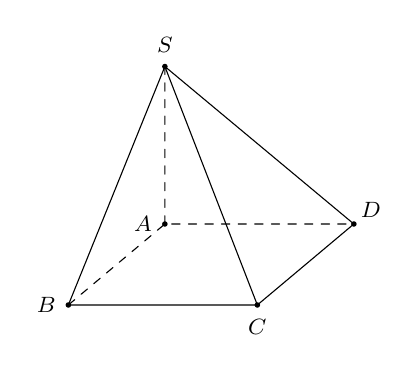
\begin{tikzpicture}[>=stealth,line join=round,line cap=round,font=\footnotesize,scale=.8]
				\path (0,0) coordinate (B)
				++(0:3) coordinate (C) 
				++(40:2)  coordinate (D)
				++(-180:3) coordinate (A)
				++(90:2.5) coordinate (S);
				\draw (B)--(C)--(D) (S)--(D) (S)--(C)  (S)--(B);
				\draw[dashed] (B)--(A)--(D) (A)--(S)  ; % nét đứt
				\foreach \x/\y in {A/-180,B/-180,C/-90,D/40,S/90
				}{\draw[fill=black] (\x) circle(1pt)++(\y:0.35)node{$\x$};}
		\end{tikzpicture}	}
	}
\end{ex}
%Câu 3
\begin{ex}%[1H8H4-3]
	\immini{Cho hình chóp $S.ABC$ có đáy $ABC$ là tam giác đều cạnh $a$, cạnh bên $SA$ vuông góc với đáy (tham khảo hình vẽ).
		Khi đó số đo góc giữa hai mặt phẳng $(SAB)$ và $(ABC)$ là
		\choice[2]
		{$45^{\circ}$}
		{\True $90^{\circ}$}
		{$30^{\circ}$}
		{$60^{\circ}$}}
	{\begin{tikzpicture}[>=stealth,line join=round,line cap=round,font=\footnotesize,scale=.8]
			\path (0,0) coordinate (A)
			++(-45:2.5) coordinate (B) 
			++(30:3)  coordinate (C)
			++(140:5.8) coordinate (S);
			\draw (A)--(B)--(C)--(S)--cycle (S)--(B);
			\draw[dashed] (A)--(C)  ; % nét đứt
			\foreach \x/\y in {A/-180,B/-90,C/40,S/90
			}{\draw[fill=black] (\x) circle(1pt)++(\y:0.35)node{$\x$};}
			\draw pic[draw, angle radius=2.5mm]{right angle=B--A--S};
			\draw pic[draw, angle radius=2.5mm]{right angle=C--A--S};
	\end{tikzpicture}	}
	\loigiai{
		Do $SA\perp(ABC)$ mà $SA\subset(SAB)$ $\Rightarrow(SAB)\perp(ABC)$.\\
		Vậy số đo góc giữa hai mặt phẳng $(SAB)$ và $(ABC)$ là $90^{\circ}$. }
\end{ex}
%Câu 4
\begin{ex}%[1H8H4-2]
	Xét hình chóp $S.ABC$ có đáy $ABC$ là tam giác vuông tại $A$, cạnh bên $SA$ vuông góc với đáy. Gọi $M$ là trung điểm của $BC$. Chọn khẳng định \textbf{sai}.
	\choice
	{\True $(SAM)\perp(SBC)$}
	{$(SAB)\perp(ABC)$}
	{$(SAC)\perp(ABC)$}
	{$(SAB)\perp (SAC)$}
	\loigiai{
		\immini{
			Ta có $SA\perp(ABC)\Rightarrow\heva{
				&(SAB)\perp(ABC)\\
				&(SAC)\perp(ABC).
			}$\\
			$\heva{
				&AB\perp AC\\
				&AB\perp SA
			}\Rightarrow (SAB)\perp (SAC)$.\\
			Vậy $(SAM)\perp(SBC)$ là khẳng định sai.}
		{\begin{tikzpicture}[>=stealth,line join=round,line cap=round,font=\footnotesize,scale=.8]
				\path (0,0) coordinate (A)
				++(90:3.5) coordinate (S) 
				++(-50:5)  coordinate (B)
				++(200:5)  coordinate (C);
				\coordinate (M) at ($(B)!0.5!(C)$);	
				\draw  (S)--(B)--(C)--cycle (S)--(B);
				\draw[dashed] (A)--(S) (A)--(B) (A)--(C) (A)--(M); % nét đứt
				\foreach \x/\y in {A/-180,B/-90,C/-180,S/90,M/-45
				}{\draw[fill=black] (\x) circle(1pt)++(\y:0.35)node{$\x$};}
				\draw pic[draw, angle radius=2.5mm]{right angle=B--A--S};
				\draw pic[draw, angle radius=2.5mm]{right angle=C--A--S};
				\draw pic[draw, angle radius=2.5mm]{right angle=C--A--B};
		\end{tikzpicture}}
	}
\end{ex}
%Câu 5
\begin{ex}%[1H8H4-3]
	\immini{
		Cho hình chóp $S.ABC$ có đáy $ABC$ là tam giác đều cạnh $a$, cạnh bên $SA$ vuông góc với đáy (tham khảo hình vẽ bên). Khi đó số đo góc giữa hai mặt phẳng $(SAB)$ và $(ABC)$ là
		\choice[2]
		{$45^{\circ}$}
		{\True $90^{\circ}$}
		{$30^{\circ}$}
		{$60^{\circ}$}
	}
	{\begin{tikzpicture}[>=stealth,line join=round,line cap=round,font=\footnotesize,scale=1]
			\path (0,0) coordinate (A)
			++(-45:2.5) coordinate (B) 
			++(30:3)  coordinate (C)
			++(140:5.8) coordinate (S);
			\draw (A)--(B)--(C)--(S)--cycle (S)--(B);
			\draw[dashed] (A)--(C)  ; % nét đứt
			\foreach \x/\y in {A/-180,B/-90,C/40,S/90
			}{\draw[fill=black] (\x) circle(1pt)++(\y:0.35)node{$\x$};}
			\draw pic[draw, angle radius=2.5mm]{right angle=B--A--S};
			\draw pic[draw, angle radius=2.5mm]{right angle=C--A--S};
		\end{tikzpicture}			
	}
	\loigiai{
		Do $SA\perp(ABC)$ mà $SA\subset(SAB)$ $\Rightarrow(SAB)\perp(ABC)$\\
		Vậy số đo góc giữa hai mặt phẳng $(SAB)$ và $(ABC)$ là $90^{\circ}$.}
\end{ex}
%Câu 6
\begin{ex}%[1H8H4-2]
	Cho hình chóp $S.ABCD$ có đáy $ABCD$ là hình thoi tâm $O$, $SO\perp (ABCD)$. Gọi $M$ là trung điểm của $SA$. Mặt phẳng $(MBD)$ vuông góc với mặt phẳng nào dưới đây?
	\choice
	{$(SBC)$}
	{\True$(SAC)$}
	{$(SBD)$}
	{$(ABCD)$}
	\loigiai{
		\immini{
			Ta có $\heva{
				&BD\perp AC\\
				&BD\perp SO (\text{vì }SO\perp (ABCD)).}$\\
			$\Rightarrow BD \perp (SAC)$ mà $BD \subset (MBD)$.\\
			Vậy $(MBD) \perp (SAC)$.}
		{	\begin{tikzpicture}[>=stealth,line join=round,line cap=round,font=\footnotesize,scale=.7]
				\path (0,0) coordinate (B)
				++(0:3.5) coordinate (C) 
				++(45:2.5)  coordinate (D)
				++(180:3.5) coordinate (A)
				++(75:4) coordinate (S);
				\coordinate (O) at (intersection of A--C and B--D); 
				\coordinate (M) at ($(S)!0.5!(A)$);
				\draw (B)--(C)--(D)--(S)--(B)--cycle (S)--(C);
				\draw[dashed] (A)--(C) (A)--(B) (A)--(S) (A)--(D) (S)--(O) (B)--(D) (B)--(M) (M)--(D) ; % nét đứt
				\foreach \x/\y in {A/-180,B/-180,C/0,S/90,D/0,O/-95,M/-80
				}{\draw[fill=black] (\x) circle(1pt)++(\y:0.35)node{$\x$};}
		\end{tikzpicture}	}
	}
\end{ex}
%Câu 7
\begin{ex}%[1H8H4-2]
	Cho hình chóp $S.ABC$ có $SA\perp(ABC)$, đáy $ABC$ là tam giác vuông tại $A$, $M$ là trung điểm $BC$. Khi đó mặt phẳng $(ABC)$ \textbf{không} vuông góc với mặt phẳng nào?
	\choice
	{$(SAB)$}
	{$(SAM)$}
	{$(SAC)$}
	{\True $(SBC)$}
	\loigiai{
		\immini{
			Ta có $SA\perp(ABC)$ (theo gt).\\
			Mà $SA\subset(SAB)\Rightarrow(SAB)\perp(ABC)$.\\
			Mà $SA\subset(SAC)\Rightarrow(SAC)\perp(ABC)$.\\
			Mà $SA\subset(SAM)\Rightarrow(SAM)\perp(ABC)$.\\
			Vậy mặt phẳng $(ABC)$ không vuông góc với mặt phẳng $(SBC)$.}
		{\begin{tikzpicture}[>=stealth,line join=round,line cap=round,font=\footnotesize,scale=1]
				\path (0,0) coordinate (A)
				++(-45:2.5) coordinate (B) 
				++(30:3)  coordinate (C)
				++(140:5.8) coordinate (S);
				\draw (A)--(B)--(C)--(S)--cycle (S)--(B);
				\draw[dashed] (A)--(C)  ; % nét đứt
				\foreach \x/\y in {A/-180,B/-90,C/40,S/90
				}{\draw[fill=black] (\x) circle(1pt)++(\y:0.35)node{$\x$};}
				\draw pic[draw, angle radius=2.5mm]{right angle=B--A--S};
				\draw pic[draw, angle radius=2.5mm]{right angle=C--A--S};
		\end{tikzpicture}		}
	}
\end{ex}
%Câu 8
\begin{ex}%[1H8N4-3]
	Cho tứ diện $ABCD$ có $AB$ vuông góc với mặt phẳng $(BCD)$, tam giác $BCD$ vuông tại $C$. Khẳng định nào sau đây đúng về góc giữa hai mặt phẳng $(ACD)$ và $(BCD)$?
	\choice
	{\True $({(ACD),(BCD)})=\widehat{ACB}$}
	{ $({(ACD),(BCD)})=\widehat{ADB}$}
	{ $({(ACD),(BCD)})=\widehat{CAB}$}
	{ $({(ACD),(BCD)})=\widehat{CBD}$}
	\loigiai{
		\immini{
			Vì tam giác $BCD$ vuông tại $C$ nên $BC\perp CD$.\\
			Vì $\heva{
				&	CD\perp BC\\
				&	CD\perp AB}$
			nên $CD\perp(ABC)$. Do đó, $CD\perp AC$.\\
			Ta có 
			$\heva{
				&	(ACD)\cap(BCD)=CD\\
				&	AC\perp CD,\,AC\subset(ACD)\\
				&	BC\perp CD,\,BC\subset(BCD)
			}\\
			\Rightarrow((ACD),(BCD))=(AC,CB)=\widehat{ACB}$.}
		{\begin{tikzpicture}[>=stealth,line join=round,line cap=round,font=\footnotesize,scale=1]
				\path (0,0) coordinate (B)
				++(-45:2.5) coordinate (C) 
				++(30:3)  coordinate (D)
				++(140:5.8) coordinate (A);
				\draw (B)--(C)--(D)--(A)--cycle (A)--(C);
				\draw[dashed] (B)--(D)  ; % nét đứt
				\foreach \x/\y in {D/0,C/-90,B/40,A/90
				}{\draw[fill=black] (\x) circle(1pt)++(\y:0.35)node{$\x$};}
		\end{tikzpicture}		}
	}
\end{ex}
%Câu 9
\begin{ex}%[1H8H4-3]
	Cho hình chóp $S.ABCD$ có đáy $ABCD$ là hình thoi cạnh $a$ và có $SA=SB=SC=a$. Góc giữa hai mặt phẳng $(SBD)$ và $(ABCD)$ bằng
	\choice
	{$30^{\circ} $}
	{\True $90^{\circ}$}
	{$60^{\circ} $}
	{$45^{\circ}$}
	\loigiai{
		\begin{center}
			\begin{tikzpicture}[>=stealth,line join=round,line cap=round,font=\footnotesize,scale=1]
				\path (0,0) coordinate (B)
				++(0:3.5) coordinate (C) 
				++(45:2.5)  coordinate (D)
				++(180:3.5) coordinate (A)
				++(100:4) coordinate (S);
				\coordinate (O) at (intersection of A--C and B--D); 
				\coordinate (H) at ($(B)!0.4!(O)$);
				\draw (B)--(C)--(D)--(S)--(B)--cycle (S)--(C);
				\draw[dashed] (A)--(C) (A)--(B) (A)--(S) (A)--(D) (S)--(H) (B)--(D) (H)--(A) (H)--(C) ; % nét đứt
				\foreach \x/\y in {A/-180,B/-180,C/0,S/90,D/0,H/150
				}{\draw[fill=black] (\x) circle(1pt)++(\y:0.35)node{$\x$};}
			\end{tikzpicture}			
		\end{center}
		Gọi $H$ là chân đường vuông góc của $S$ xuống mặt phẳng đáy $(ABCD)$.\\
		Suy ra $SH\perp(ABCD)$.\\
		Vì $SA=SB=SC=a$ nên các hình chiếu $HA=HB=HC$. Do đó, $H$ là tâm đường tròn ngoại tiếp $(ABC)$.\\
		Mà tam giác $ABC$ cân tại $B$ (vì $BA=BC=a$) nên tâm $H$ phải nằm trên $BD$, ta có $SH\subset(SBD)$.\\
		Vậy có $\heva{
			&SH\perp(ABCD)\\
			&SH\subset(SBD)}$
		$\Rightarrow(SBD)\perp(ABCD)$ nên góc $({(SBD),(ABCD)})=90^{\circ}$. \\
	}
\end{ex}
%Câu 10
\begin{ex}%[1H8V4-3]
	Cho tứ diện đều $ABCD$ có tất cả các cạnh đều bằng $a$. Tính cosin góc giữa hai mặt phẳng $(ABC)$ và $(BCD)$.
	\choice
	{$\cos\alpha =\dfrac{1}{6}$}
	{\True $\cos\alpha =\dfrac{1}{3}$}
	{$\cos\alpha =\dfrac{1}{4}$}
	{$\cos\alpha =\dfrac{1}{2}$}
	\loigiai{
		\begin{center}
			\begin{tikzpicture}[>=stealth,line join=round,line cap=round,font=\footnotesize,scale=1]
				\path (0,0) coordinate (B)
				++(-50:3) coordinate (C) 
				++(45:3)  coordinate (D)
				++(135:3) coordinate (A);
				\coordinate (E) at ($(B)!0.5!(C)$);
				\draw (B)--(C)--(D)--(A)--cycle (A)--(E) (A)--(C);
				\draw[dashed] (B)--(D) (D)--(E)  ; % nét đứt
				\foreach \x/\y in {A/90,B/-180,C/-90,D/0,E/-180
				}{\draw[fill=black] (\x) circle(1pt)++(\y:0.35)node{$\x$};}
			\end{tikzpicture}			
		\end{center}
		Gọi $E$ là trung điểm của $BC$\\
		Có	$\heva{&(ACB) \cap (BCD)=BC\\
			& AE \subset (ABC), AE\perp BC\\
			& DE \subset (BCD),DE\perp BC}
		\Rightarrow((ABC),(BCD))=(AE,DE)$.\\
		Do $ABCD$ là tứ diện đều cạnh $a$ nên $AE=ED=\dfrac{a\sqrt{3}}{2}$.\\
		Áp dụng định lý cosin cho tam giác $AED$ ta có \\
		$AD^2=AE^2+ED^2-2AE\cdot ED\cdot 
		\cos AED$ $\Rightarrow \cos AED=\dfrac{AE^2+ED^2-AD^2}{2\cdot AE\cdot ED}=\dfrac{1}{3}$.\\
		Gọi $\alpha$ là góc giữa hai măt phẳng $(ABC)$ và $BCD$. Suy ra $\cos\alpha=\cos \widehat{AED}=\dfrac{1}{3}$.    
	}
\end{ex}
%Câu 11
\begin{ex}%[1H8V4-3]
	Cho tam giác $ABC$ vuông cân tại $B$ và $AB=a$. Trên đường thẳng qua $A$ vuông góc với $(ABC)$ lấy điểm $S$ sao cho $SA=a$. Tính số đo góc giữa hai mặt phẳng $(SBC)$ và $(ABC)$.
	\choice
	{\True $45^\circ$}
	{$30^\circ$}
	{$60^\circ$}
	{$90^\circ$}
	\loigiai{
		\immini{	Vì tam giác $ABC$ vuông tại $B$ nên $BC \perp AB$.\\
			Vì $\heva{&BC \perp AB\\ &BC \perp SA} \Rightarrow BC \perp (SAB)$. Do đó $BC \perp SB$.\\
			Ta có\\
			$\heva{&(SBC) \cap (ABC)=BC\\ &AB \perp BC, \, AB \subset (ABC)\\ &SB \perp BC, \, SB \subset (SBC)} \Rightarrow ((SBC), (ABC))=(SB, AB) =\widehat{SBA}$.\\
			Tam giác $SAB$ vuông tại $A$ ta có \\
			$\tan {SBA} =\dfrac{SA}{AB}=1$, suy ra $\widehat{SBA}=45^\circ$.}
		{\begin{tikzpicture}[>=stealth,line join=round,line cap=round,font=\footnotesize,scale=1]
				\path (0,0) coordinate (A)
				++(-45:2.5) coordinate (C) 
				++(30:3)  coordinate (B)
				++(140:5.8) coordinate (S);
				\draw (A)--(C)--(B)--(S)--cycle (S)--(C);
				\draw[dashed] (A)--(B)  ; % nét đứt
				\foreach \x/\y in {B/0,C/-90,A/-90,S/90
				}{\draw[fill=black] (\x) circle(1pt)++(\y:0.35)node{$\x$};}
		\end{tikzpicture}}
	}
\end{ex}
%Câu 12
\begin{ex}%[1H8V4-3]
	CHo lăng trụ đứng $ABC.A'B'C'$ có đáy $ABC$ là tam giác vuông cân tại $A$, $AB=a$. Biết thể tích khối lăng trụ $ABC.A'B'C'$ bằng $\dfrac{a^3\sqrt{6}}{12}$. Góc giữa hai mặt phẳng $(A'BC)$ và $(ABC)$ bằng
	\choice
	{\True $30^\circ$}
	{$90^\circ$}
	{$60^\circ$}
	{$45^\circ$}
	\loigiai
	{
		\immini{Ta có $$V=S_{ABC}\cdot AA' \Leftrightarrow \dfrac{a^3\sqrt{6}}{12} =\dfrac{1}{2}a^2AA' \Rightarrow AA'=\dfrac{\sqrt{6}}{6}a.$$
			Dựng $AI \perp BC$ ta suy ra $BC \perp (A'AI)$.\\
			Ta có 
			$\heva{&(A'BC) \cap (ABC) =BC\\ &BC \perp(A'AI)\\ &(A'AI) \cap (A'BC)=A'I\\ &(A'AI) \cap (ABC)=AI}\\ \Rightarrow ((A'BC),(ABC))=(A'I,AI)=\widehat{A'IA}$.\\
			Ta có $\tan {A'IA}=\dfrac{A'A}{AI}=\dfrac{\dfrac{\sqrt{6}}{6}a}{\dfrac{a\sqrt{2}}{2}}=\dfrac{\sqrt{3}}{3} \Rightarrow \widehat{A'IA}=30^\circ$.}
		{\begin{tikzpicture}[>=stealth,line join=round,line cap=round,font=\footnotesize,scale=1]
				\path (0,0) coordinate (A)
				++(-50:3) coordinate (B) 
				++(50:3.1)  coordinate (C)
				++(90:4.5) coordinate (C')
				++(-180:4.1) coordinate (A')
				++(-40:3) coordinate (B');
				\coordinate (M) at ($(B)!0.5!(C)$);	
				\draw (A)--(B)--(C)--(C')--(A')--cycle (A')--(B')  (C')--(B') (B)--(B')(A')--(B) ;
				\draw[dashed] (A)--(C)  (A)--(M) (A')--(M) (A')--(C); % nét đứt
				\foreach \x/\y in {A/-180,B/-90,C/0,{C'}/45,{A'}/-180,{B'}/-135,M/-30
				}{\draw[fill=black] (\x) circle(1pt)++(\y:0.35)node{$\x$};}
				\draw pic[draw, angle radius=2.5mm]{right angle={A'}--A--M};
				\draw pic[draw, angle radius=2.5mm]{right angle=A--M--B};
				\draw pic[draw, angle radius=2.5mm]{right angle=B--A--C};
		\end{tikzpicture}	}
	}
\end{ex}
\Closesolutionfile{ans}
\indapan{6}{ans/ans-1C8B3-De1}
\cauds
\Opensolutionfile{ans}[ans/ans-1C8B3-De1-DS]
\begin{ex}%[1H8V4-3]
	Cho hình chóp $S.ABCD$ có đáy là hình chữ nhật với $AB=a$, $AD=a\sqrt{3}$. Biết $SA$ vuông góc với mặt phẳng đáy và $SA=a\sqrt {3}$. 
	\choiceTF
	{\True $((SAB),(ABCD))=90^{\circ}$}
	{$((SBC),(ABCD))=\widehat{SAB}$}
	{\True $((SBC),(ABCD))=60^{\circ}$}
	{$((SBD),(ABCD))\approx 69{,}43^{\circ}$}
	\loigiai{
		\begin{center}
			\begin{tikzpicture}[>=stealth,line join=round,line cap=round,font=\footnotesize,scale=1]
				\path (0,0) coordinate (B)
				++(0:4) coordinate (C) 
				++(45:2.5)  coordinate (D)
				++(180:4) coordinate (A)
				++(90:3) coordinate (S);
				\coordinate (K) at ($(B)!0.45!(D)$);	 
				\draw (B)--(C)--(D)--(S)--(B)--cycle (S)--(C);
				\draw[dashed] (A)--(B) (A)--(S) (A)--(D) (B)--(D) (S)--(K) (A)--(K) ; % nét đứt
				\foreach \x/\y in {A/-180,B/-180,C/0,S/90,K/0,D/0
				}{\draw[fill=black] (\x) circle(1pt)++(\y:0.35)node{$\x$};}
				\draw pic[draw, angle radius=2.5mm]{right angle=S--A--D};
				\draw pic[draw, angle radius=2.5mm]{right angle=B--A--D};
				\draw pic[draw, angle radius=2.5mm]{right angle=A--K--B};
			\end{tikzpicture}			
		\end{center}
		\begin{itemchoice}
			\itemch {Đúng}. Vì  $\heva{
				&SA\perp (ABCD)\\
				&SA\subset (SAB)}$
			$\Rightarrow (SAB)\perp (ABCD)$.\\
			Hay $((SAB),(ABCD))=90^{\circ}$.
			\itemch {Sai}. $\heva{
				&BC\perp AB\\
				&BC\perp SA(\text{do }SA\perp (ABCD))}
			\Rightarrow BC\perp (SAB)\Rightarrow BC\perp SB$.\\
			Khi đó $\heva{
				&BC=(SBC)\cap (ABCD)\\
				&AB\perp BC,SB\perp BC\\
				&AB\subset (ABCD),SB\subset (SBC).}$\\
			$\Rightarrow ((SBC),(ABCD))=(SB,AB)=\widehat{SBA}$ (góc $\widehat{SBA}$ nhọn vì $\widehat{SAB}=90^{\circ}$).
			\itemch {Đúng}. Vì
			tam giác $SAB$ vuông tại $A$ có $\tan\widehat{SBA}=\dfrac{SA}{AB}=\dfrac{a\sqrt {3}}{a}=\sqrt{3}$.\\ $\Rightarrow\widehat{SBA}=60^{\circ}$.\\
			Vậy $((SBC),(ABCD))=\widehat{SBA}=60^{\circ}$.
			\itemch {Sai}.
			Kẻ đường cao $AK$ của tam giác $ABD$\\
			Ta có $\heva{
				&BD\perp AK\\
				&BD\perp SA}
			\Rightarrow BD\perp (SAK) \Rightarrow BD\perp SK$.\\
			Khi đó $\heva{
				&(SBD)\cap (ABCD)=BD\\
				&AK\perp BD,SK\perp BD\\
				&AK\subset (ABCD),SK\subset (SBD).}$\\
			$\Rightarrow ((SBD),(ABCD))=(SK,AK)=\widehat{SKA}$ (góc $\widehat{SKA}$ nhọn vì $\widehat{SAK}=90^{\circ}$).\\
			Tam giác $ABD$ vuông tại $A$ có đường cao $AK$ nên\\
			$\dfrac{1}{AK^2}=\dfrac{1}{AB^2}+\dfrac{1}{AD^2}=\dfrac{1}{a^2}+\dfrac{1}{3a^2}=\dfrac{4}{3a^2}\Rightarrow AK=\dfrac{a\sqrt{3}}{2}$.\\
			Tam giác $SAK$ vuông tại $A$ có $\tan\widehat{SKA}=\dfrac{SA}{AK}=\dfrac{a\sqrt 3}{\dfrac{a\sqrt {3}}{2}}=2\Rightarrow\widehat{SKA}\approx63,43^{\circ}$.\\
			Vậy $((SBD),(ABCD))=\widehat{SKA}\approx63,43^{\circ}$.
		\end{itemchoice}
	}
\end{ex}
%Câu 2
\begin{ex}%[1H8V4-3]
	Cho hình chóp tứ giác đều $S.ABCD$ có cạnh đáy bằng $a$, tâm của đáy là $O$ với $SO=\dfrac{a\sqrt 3}{2}$. Gọi $M$, $N$ lần lượt là trung điểm cạnh $AD$ và $BC$.
	\choiceTF
	{\True $(SMN)\perp (ABCD)$}
	{\True $(SAD)\perp (SMN)$}
	{$((SBC),(ABCD))=30^{\circ}$}
	{$((SBC),(SCD))\approx 80{,}52^{\circ}$}		
	\loigiai{
		\begin{center}
			\begin{tikzpicture}[>=stealth,line join=round,line cap=round,font=\footnotesize,scale=1]
				\path (0,0) coordinate (D)
				++(0:5) coordinate (C) 
				++(50:3)  coordinate (B)
				++(180:5) coordinate (A)
				++(75:4.5) coordinate (S);
				\coordinate (O) at (intersection of A--C and B--D); 
				\coordinate (I) at ($(S)!0.6!(C)$);	
				\coordinate (M) at ($(A)!0.5!(D)$); 
				\coordinate (N) at ($(B)!0.5!(C)$);
				\draw (D)--(C)--(B)--(S)--cycle (S)--(C) (I)--(D) (I)--(B) (S)--(N);
				\draw[dashed] (A)--(B) (A)--(S) (A)--(D) (B)--(D) (A)--(C) (M)--(N) (O)--(I) (S)--(M) (S)--(O); % nét đứt
				\foreach \x/\y in {A/45,B/0,C/0,S/90,O/-90,D/-180,M/-45,N/0,I/45
				}{\draw[fill=black] (\x) circle(1pt)++(\y:0.35)node{$\x$};}
				\draw pic[draw, angle radius=2.5mm]{right angle=S--O--A};
				\draw pic[draw, angle radius=2.5mm]{right angle=D--I--C};
			\end{tikzpicture}			
		\end{center}
		\begin{itemchoice}
			\itemch {Đúng}. Vì $S.ABCD$ là hình chóp tứ giác đều có $O$ là tâm của đáy nên $SO\perp (ABCD)$ Mặt khác $MN$ là đường trung bình của hình vuông $ABCD$ nên $MN$ qua $O$.\\
			Vậy $SO\subset (SMN)\Rightarrow(SMN)\perp (ABCD)$.
			\itemch {Đúng}. Vì ta có $\heva{
				&AD\perp MN\\
				&AD\perp SO
			}\Rightarrow AD\perp (SMN)$.\\
			mà $AD\subset (SAD)\Rightarrow(SAD)\perp (SMN)$.
			\itemch {Sai}. Vì ta có $\heva{
				&BC\parallel AD\\
				&AD\perp (SMN)
			}$
			$\Rightarrow BC\perp (SMN)\Rightarrow BC\perp MN$.\\
			Khi đó $\heva{
				&(SBC)\cap (ABCD)=BC\\
				&ON\perp BC,SN\perp BC\\
				&ON\subset (ABCD),SN\subset (SBC).}
			$\\
			$\Rightarrow((SBC),(ABCD))=(SN,ON)=\widehat{SNO}$\\
			Vì $ON$ là đường trung bình tam giác $ABC$ nên $ON=\dfrac{AB}{2}=\dfrac{a}{2}$.\\
			Tam giác $SON$ vuông tại $O$ có\\ $\tan\widehat{SNO}=\dfrac{SO}{ON}=\dfrac{\dfrac{a\sqrt 3}{2}}{\dfrac{a}{2}}=\sqrt 3\Rightarrow\widehat{SNO}=60^{\circ}$\\
			Vậy $((SBC),(ABCD))=\widehat{SNO}=60^{\circ}$.
			\itemch {Sai}. Vì
			Kẻ đường cao $DI$ của tam giác $SCD$\\
			Ta có $\heva{
				&SC\perp DI\\
				&SC\perp BD(\text{do }BD\perp (SAC))}$
			$\Rightarrow SC\perp (IBD)\Rightarrow SC\perp BI$.\\
			Mặt khác $SC=(SBC)\cap (SCD)$ nên $((SBC),(SCD))=(ID,IB)$\\
			Ta có $\heva{
				&BC\parallel AD\\
				&AD\perp (SMN)}$
			$\Rightarrow BC\perp (SMN)\Rightarrow BC\perp MN$.\\
			Khi đó $\heva{
				&(SBC)\cap (ABCD)=BC\\
				&ON\perp BC,SN\perp BC\\
				&ON\subset (ABCD),SN\subset (SBC).}$\\
			$\Rightarrow((SBC),(ABCD))=(SN,ON)=\widehat{SNO}$.\\
			Vì $ON$ là đường trung bình tam giác $ABC$ nên $ON=\dfrac{AB}{2}=\dfrac{a}{2}$.\\
			Tam giác $SON$ vuông tại $O$ có $\tan\widehat{SNO}=\dfrac{SO}{ON}=\dfrac{\dfrac{a\sqrt 3}{2}}{\dfrac{a}{2}}=\sqrt 3 \Rightarrow\widehat{SNO}=60^{\circ}$.\\
			Vậy $((SBC),(ABCD))=\widehat{SNO}=60^{\circ}$.\\
			Kẻ đường cao $DI$ của tam giác $SCD$.\\
			Ta có $\heva{
				&SC\perp DI\\
				&SC\perp BD(\text{do }BD\perp (SAC))}$
			$\Rightarrow SC\perp (IBD)\Rightarrow SC\perp BI$.\\
			Mặt khác $SC=(SBC)\cap (SCD)$ nên $((SBC),(SCD))=(ID,IB)$.\\
			Ta có $IO\perp BD$ và $O$ là trung điểm $BD$.\\
			nên $\Delta IBD$ cân tại $I$ và $\widehat{OIB}=\widehat{OID}=\dfrac{1}{2}\widehat{BID}$.\\
			Vì $ABCD$ là hình vuông cạnh $a$ nên $OC=\dfrac{AC}{2}=\dfrac{a\sqrt 2}{2}=OD$.\\
			Tam giác $SOC$ có đường cao\\
			$OI=\dfrac{SO\cdot OC}{\sqrt{S{O^2}+O{C^2}}}=\dfrac{a\sqrt{30}}{10}$\\
			Tam giác $IOD$ vuông tại $O$ có\\
			$\tan\widehat{OID}=\dfrac{OD}{OI}=\dfrac{\dfrac{a\sqrt 2}{2}}{\dfrac{a\sqrt{30}}{10}}=\dfrac{\sqrt{15}}{3}$;\\ $\tan\widehat{BID}=\dfrac{2\tan\widehat{OID}}{1-\tan^2\widehat{OID}}=-\sqrt{15}< 0$ nên $\widehat{BID}$ là góc tù.\\
			Vậy $((SBC),(SCD))=(ID,IB)=180^{\circ}-\widehat{BID}\approx75,52^{\circ}$.
		\end{itemchoice}	
	}
\end{ex}
%Câu 3
\begin{ex}%[1H8H4-3]
	Cho hình chóp $S.ABCD$ có đáy $ABCD$ là hình vuông, $SA\perp (ABCD)$. 
	\choiceTF
	{\True $((SAC),(SBD))=90^{\circ}$}
	{\True $((SAC),(SAD))=45^{\circ}$}
	{\True $(SAB)\perp (SBC)$}
	{\True $(SCD)\perp (SAD)$}
	\loigiai{
		\begin{center}
			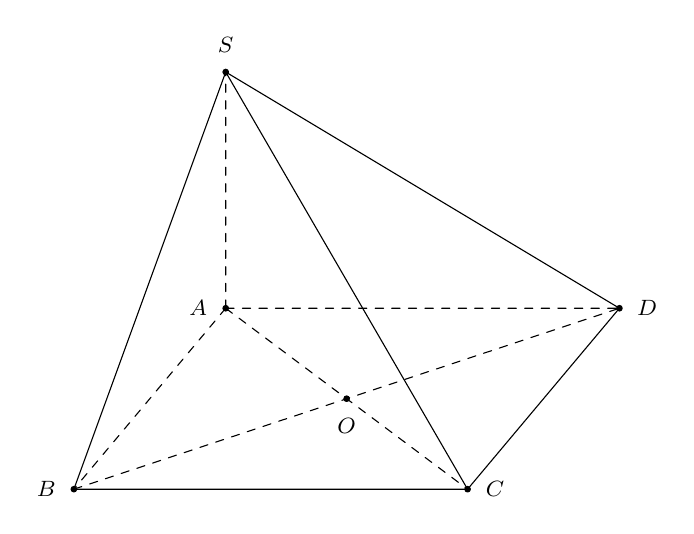
\begin{tikzpicture}[>=stealth,line join=round,line cap=round,font=\footnotesize,scale=1]
				\path (0,0) coordinate (B)
				++(0:5) coordinate (C) 
				++(50:3)  coordinate (D)
				++(180:5) coordinate (A)
				++(90:3) coordinate (S);
				\coordinate (O) at (intersection of A--C and B--D); 
				\draw (B)--(C)--(D)--(S)--cycle (S)--(C);
				\draw[dashed] (A)--(B) (A)--(S) (A)--(D) (B)--(D) (A)--(C); % nét đứt
				\foreach \x/\y in {A/-180,B/-180,C/0,S/90,O/-90,D/0
				}{\draw[fill=black] (\x) circle(1pt)++(\y:0.35)node{$\x$};}
			\end{tikzpicture}			
		\end{center}
		\begin{itemchoice}
			\itemch {Đúng}. Vì $\heva{
				&BD\perp (SAC)\\
				&BD\subset (SBD)}$
			$\Rightarrow (SAC)\perp (SBD)$.\\
			\itemch {Đúng}.  Vì $\heva{
				&AC\perp SA\\
				&AD\perp SA\\
				&AC\subset (SAC), AD\subset(SAD)\\
				& (SAC)\cap (SAD)=SA.}$ \\$ \Rightarrow ((SAC),(SAD))=(AC,AD)=\widehat{CAD}=45^{\circ}$.
			\itemch {Đúng}. Vì $\heva{
				&BC\perp (SAB)&\\
				&BC\subset (SBC)}$
			$\Rightarrow (SAB)\perp (SBC)$.
			\itemch {Đúng}. Vì $\heva{
				&CD\perp (SAD)\\
				&CD\subset (SCD)}$
			$\Rightarrow (SAD)\perp (SCD)$. 
		\end{itemchoice}
	}
\end{ex}
%Câu 4
\begin{ex}%[1H8H4-3]
	Cho hình chóp $S.ABC$ có đáy là tam giác $ABC$ vuông tại $A$ và $I\perp (ABC)$. 
	\choiceTF
	{\True  $(SAC)\perp (ABC)$}
	{\True Gọi $H$ là hình chiếu của $A$ trên $BC$. Khi đó $(SAH)\perp (SBC)$}
	{$(AB,SC)=60^{\circ}$}
	{Gọi $K$ là hình chiếu của $A$ trên $SC$. Khi đó $((ABK),(SBC))=60^{\circ} $}
	\loigiai{
		\begin{center}
			\begin{tikzpicture}[>=stealth,line join=round,line cap=round,font=\footnotesize,scale=1]
				\path (0,0) coordinate (A)
				++(-55:2.5) coordinate (B) 
				++(30:4)  coordinate (C)
				++(145:5.7) coordinate (S);
				\coordinate (H) at ($(B)!0.35!(C)$);	
				\coordinate (K) at ($(S)!0.4!(C)$);	
				\draw (A)--(B)--(C)--(S)--cycle (S)--(B) (K)--(B) ;
				\draw[dashed] (A)--(C)  (A)--(K) (A)--(H); % nét đứt
				\foreach \x/\y in {A/-180,B/-90,C/40,S/90,H/-45,K/90
				}{\draw[fill=black] (\x) circle(1pt)++(\y:0.35)node{$\x$};}
				\draw pic[draw, angle radius=2.5mm]{right angle=B--A--S};
				\draw pic[draw, angle radius=2.5mm]{right angle=C--A--S};
				\draw pic[draw, angle radius=2.5mm]{right angle=A--K--S};
				\draw pic[draw, angle radius=2.5mm]{right angle=B--K--C};
				\draw pic[draw, angle radius=2.5mm]{right angle=A--H--B};
			\end{tikzpicture}			
		\end{center}
		\begin{itemchoice}
			\itemch \textbf{Đúng}. Vì
			$\heva{
				&SA\perp (ABC)\\
				&(SAC)\supset SA}
			\Rightarrow (SAC)\perp (ABC)$.
			\itemch \textbf{Đúng}. Vì  $\heva{
				&BC\perp (SAH)\\
				&(SBC)\supset BC}
			\Rightarrow (SBC)\perp (SAH).$
			\itemch \textbf{Sai}. Vì $AK\perp SC$ và $AB\perp (SAC)\Rightarrow AB\perp SC$, nên $SC\perp (ABK).$ 
			\itemch \textbf{Sai}. Vì ta có $\heva{
				&SC\perp (ABK)\\
				&(SBC)\supset SC}
			\Rightarrow (SBC)\perp (ABK)$.
		\end{itemchoice}
	}
\end{ex}
\Closesolutionfile{ans}
\indapan{3}{ans/ans-1C8B3-De1-DS}
\caukq
\Opensolutionfile{ans}[ans/ans-1C8B3-De1-KQ]
%Câu 1
\begin{ex}%[1H8V4-3]
	Cho hình lập phương $ABCD.A'B'C'D'$. Tính góc giữa hai mặt phẳng $(AB'C')$ và $(AC'D')$.
	\shortans{$60^\circ$}
	\loigiai{
		\begin{center}
			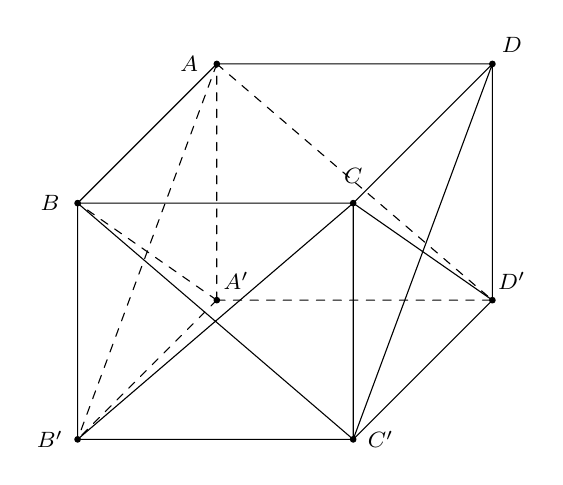
\begin{tikzpicture}[>=stealth,line join=round,line cap=round,font=\footnotesize,scale=1]
				\path (0,0) coordinate (B')
				++(0:3.5) coordinate (C') 
				++(45:2.5)  coordinate (D')
				++(180:3.5) coordinate (A')
				++(90:3) coordinate (A)
				++(0:3.5) coordinate (D)
				++(-135:2.5) coordinate (C)
				++(-180:3.5) coordinate (B);
				\coordinate (I) at (intersection of A--B' and B--A'); 
				\coordinate (K) at (intersection of C--D' and D--C');
				\coordinate (L) at (intersection of B--C' and C--B');
				\draw (B)--(C)--(D)--(A)--(B) (B)--(B')--(C')--(D')--(D) (C')--(C) (B)--(B') (C)--(D') (D)--(C') (B)--(C') (C)--(B');
				\draw[dashed] (A')--(A) (A')--(B') (A')--(B') (A')--(B) (A)--(D') (A')--(D') (A)--(B') (A)--(B'); % nét đứt
				\foreach \x/\y in {A/-180,B/-180,C/90,D/45,{A'}/45,{D'}/45,{C'}/0,{B'}/-180
				}{\draw[fill=black] (\x) circle(1pt)++(\y:0.35)node{$\x$};}
			\end{tikzpicture}			
		\end{center}
		Vì $ABCD\cdot A'B'C'D'$ là hình lập phương nên $BC\perp(ABB'A')\Rightarrow BC\perp AB'$. \qquad(1)\\
		Mặt khác $A'B\perp AB'$ (hai đường chéo trong hình vuông). \qquad(2)\\
		Từ $(1)$ và $(2)$ suy ra $AB'\perp(BCD'A')$.\\
		Mà $A{B'}\subset(ADC'B')$ nên $(ADC'B')\perp(BCD'A')$.\\
		Nhận xét $(AB'C')\equiv(ADC'B'),(AC'D')\equiv(ABC'D')$.\\
		Ta có $\heva{
			&CD'\bot C'D\\
			&CD'\perp AD \, (\text{do }AD\perp(CDD'C'))}
		\Rightarrow CD'\perp(ADC'B')$ \qquad(3)\\
		Tương tự $\heva{
			&B'C\perp BC'\\
			&B'C\perp AB(\text{do }AB\perp(BCC'B'))}
		\Rightarrow B'C\perp(ABC'D')$. \qquad(4)\\
		Từ $(3)$ và $(4)$ suy ra $((AB'C'),(AC'D'))=(CD',CB')$.\\
		Giả sử cạnh hình lập phương bằng $a$.\\
		Ta có $CB'=CD'=B'D'=a\sqrt{2}$ (đường chéo trong hình vuông).\\
		Suy ra tam giác $CB'D'$ đều.\\
		Do vậy $((AB'C'),(AC'D'))=(C{D'},C{B'})=\widehat{B'CD'}=60^{\circ}$.				
	}
\end{ex}
%Câu 2
\begin{ex}%[1H8V4-3]
	Cho hình chóp $S.ABCD$ có đáy $ABCD$ là hình chữ nhật $AB=a$, $AD=a\sqrt{3}$. Cạnh bên $SA$ vuông góc với đáy và $SA=a$. Gọi $\alpha=((SCD),(ABCD))$ và $\beta = ((SBC),(SAD))$. Khi đó $\alpha + \beta$ bằng.
	\shortans{$75^\circ$}
	\loigiai{
		\begin{center}
			\begin{tikzpicture}[>=stealth,line join=round,line cap=round,font=\footnotesize,scale=1]
				\path (0,0) coordinate (B)
				++(0:5) coordinate (C) 
				++(50:3)  coordinate (D)
				++(180:5) coordinate (A)
				++(90:3) coordinate (S)
				++(0:4) coordinate (M)
				++(0:-5) coordinate (N);
				\coordinate (x) at (5.5,5.3);
				\draw (B)--(C)--(D)--(S)--cycle (S)--(C) (N)--(M);
				\draw[dashed] (A)--(B) (A)--(S) (A)--(D); % nét đứt
				\foreach \x/\y in {A/-180,B/-180,C/0,S/90,D/0
				}{\draw[fill=black] (\x) circle(1pt)++(\y:0.35)node{$\x$};}
				\draw pic[draw, angle radius=2.5mm]{right angle=S--A--B};
				\path (x)node [above]{$x$};
			\end{tikzpicture}			
		\end{center}
		$\heva{
			&CD\perp AD\\
			&CD\perp SA (\text{do }SA\perp (ABCD))}$
		$\Rightarrow CD\perp (SAD)\Rightarrow CD\perp SD$.\\
		$\heva{
			&(SCD)\cap (ABCD)=CD\\
			&AD\perp CD, \, SD\perp CD\\
			&AD\subset (ABCD),SD\subset (SCD).}$
		$\Rightarrow ((SCD),(ABCD))=(SD,AD)=\widehat{SDA}$.\\
		Tam giác $SAD$ vuông tại $A$ có\\
		$\tan\widehat{SDA}=\dfrac{SA}{AD}=\dfrac{a}{a\sqrt {3}}=\dfrac{\sqrt {3}}{3}\Rightarrow\widehat{SDA}=30^{\circ}$.\\
		Vậy $((SCD),(ABCD))=\widehat{SDA}=30^{\circ}$ .\\
		Ta có $\heva{
			&S\in (SAD)\cap (SBC)\\
			&AD\parallel BC\\
			&AD\subset (SAD),BC\subset (SBC)}$
		$\Rightarrow (SAD)\cap (SBC)=S_x\parallel AD\parallel BC$.\\
		Ta có $\heva{
			&SA\perp AD\\
			&Sx\parallel AD}\Rightarrow SA\perp S_x$. \\
		Lại có $\heva{
			&S_x\perp SA\\
			&S_x\perp AB (\text{do }S_x\parallel AD,AD\perp AB)}$
		$\Rightarrow S_x\perp (SAB)\Rightarrow S_x\perp SB$.\\
		Khi đó $\heva{
			&(SBC)\cap (SAD)=S_x\\
			&SB\perp S_x,SA\perp S_x\\
			&SB\subset (SBC),SA\subset (SAD)}$
		$\Rightarrow ((SBC),(SAD))=(SB,SA)=\widehat{ASB}$.\\
		Tam giác $SAB$ vuông cân tại $A$ nên $\widehat{ASB}=45^{\circ}$.\\
		Vậy $((SBC),(SAD))=\widehat{ASB}=45^{\circ}$.
	}
\end{ex}
%Câu 3
\begin{ex}%[1H8V4-3]
	Cho hình chóp $S.ABC$ có đáy $ABC$ là tam giác vuông tại $B$. Cạnh bên $SA$ vuông góc với mặt phẳng đáy. Góc giữa mặt phẳng $(SBC)$ và mặt phẳng $(ABC)$  là $\widehat{xyz}$, (theo bảng $24$ chữ cái tiếng anh) gọi $a$ là thứ tự của chữ cái $x$, $b$ là thứ tự của chữ cái $y$, $c$ là thứ tự của chữ cái $z$. Hãy tính tống $a+b+c$.
	\shortans{$22$}
	\loigiai{
		\immini{
			Do $AB$ là hình chiếu của $SB$ trên $(ABC)$ mà $AB\perp BC\Rightarrow SB\perp BC$ (định lí 3 đường vuông góc).\\
			Ta có $\heva{
				&(SBC)\cap (ABC)=BC\\
				&SB\subset (SBC);SB\perp BC\\
				&AB\subset (ABC);AB\perp BC.}$\\
			Góc giữa mặt phẳng $(SBC)$ và mặt phẳng $(ABC)$ là $(SB,AB)=\widehat{SBA}$.\\
			Theo bảng chữ cái $a=19$, $b=2$, $c=1$.\\
			Vậy $a+b+c=22$.}
		{	\begin{tikzpicture}[>=stealth,line join=round,line cap=round,font=\footnotesize,scale=1]
				\path (0,0) coordinate (A)
				++(-45:2.5) coordinate (B) 
				++(30:3)  coordinate (C)
				++(140:5.8) coordinate (S);
				\draw (A)--(B)--(C)--(S)--cycle (S)--(B);
				\draw[dashed] (A)--(C)  ; % nét đứt
				\foreach \x/\y in {A/-180,B/-90,C/40,S/90
				}{\draw[fill=black] (\x) circle(1pt)++(\y:0.35)node{$\x$};}
				\draw pic[draw, angle radius=2.5mm]{right angle=B--A--S};
				\draw pic[draw, angle radius=2.5mm]{right angle=C--A--S};
				\draw pic[draw, angle radius=2.5mm]{right angle=A--B--C};
		\end{tikzpicture}}
	}
\end{ex}
%Câu 4
\begin{ex}%[1H8H4-3]
	Cho hình chóp $S.ABCD$ có đáy $ABCD$ là hình vuông và $SA$ vuông góc với mặt phẳng $(ABCD)$. Góc giữa hai mặt phẳng $(SCD)$ và $(ABCD)$ là $\widehat{mnq}$, (theo bảng $24$ chữ cái tiếng anh) gọi $m$ là thứ tự của chữ cái $x$, $n$ là thứ tự của chữ cái $y$, $q$ là thứ tự của chữ cái $z$. Hãy tính tống $m+n+q$.
	\shortans{$24$}
	\loigiai{
		\immini{
			$(SCD)\cap (ABCD)=CD$.\\
			Ta có $\heva{
				&{CD\perp AD}\\
				&{CD\perp SA}}
			\Rightarrow CD\perp SD$.\\
			nên góc giữa hai mặt phẳng $(SCD)$ và $(ABCD)$ là góc giữa $AD$ và $SD$ là góc $\widehat{SDA}$.\\
			Theo bảng chữ cái $m=19$, $n=4$, $q=1$.\\
			Vậy $m+n+q=24$.}
		{	\begin{tikzpicture}[>=stealth,line join=round,line cap=round,font=\footnotesize,scale=0.9]
				\path (0,0) coordinate (B)
				++(0:5) coordinate (C) 
				++(50:2.5)  coordinate (D)
				++(180:5) coordinate (A)
				++(90:3.5) coordinate (S);
				\draw (B)--(C)--(D)--(S)--cycle (S)--(C);
				\draw[dashed] (A)--(B) (A)--(S) (A)--(D); % nét đứt
				\foreach \x/\y in {A/-180,B/-180,C/0,S/90,D/0
				}{\draw[fill=black] (\x) circle(1pt)++(\y:0.35)node{$\x$};}
				\draw pic[draw, angle radius=2.5mm]{right angle=S--A--B};
	\end{tikzpicture}	}}
\end{ex}
%Câu 5
\begin{ex}%[1H8H4-3]
	Cho hình chóp $S.ABC$ có $SA\perp (ABC),SA=1$ và đáy $ABC$ là tam giác đều với độ dài cạnh bằng $2$. Tính góc giữa mặt phẳng $(SBC)$ và mặt phẳng $(ABC)$.
	\shortans{$30^\circ$}
	\loigiai{
		\immini{
			Gọi $I$ là trung điểm của $BC$ . Khi đó, ta có\\
			$\heva{
				&BC\perp SA\\
				&BC\perp AI}\Rightarrow BC\perp (SIA)\Rightarrow BC\perp SI$.\\
			Ta có 
			$\heva{
				&(SBC)\cap (ABC)=BC\\
				&SI\perp BC\\
				&AI\perp BC\\
				&SI\subset (SBC)\\
				&AI\subset (ABC)}$\\
			$\Rightarrow ((SBC),(ABC))=(SI,AI)=\widehat{SIA}$.\\
			Nên $\tan\widehat{SIA}=\dfrac{SA}{IA}=\dfrac{1}{\sqrt 3}$.\\
			Suy ra $\widehat{SIA}=30^{\circ}$ nên $\widehat{((SBC),(ABC))}=30^{\circ}$.}
		{	\begin{tikzpicture}[>=stealth,line join=round,line cap=round,font=\footnotesize,scale=1]
				\path (0,0) coordinate (A)
				++(-55:2.5) coordinate (B) 
				++(30:4)  coordinate (C)
				++(145:5.7) coordinate (S);
				\coordinate (I) at ($(B)!0.5!(C)$);	
				\draw (A)--(B)--(C)--(S)--cycle (S)--(I)  (S)--(B);
				\draw[dashed] (A)--(C)  (A)--(I); % nét đứt
				\foreach \x/\y in {A/-180,B/-90,C/40,S/90,I/-45
				}{\draw[fill=black] (\x) circle(1pt)++(\y:0.35)node{$\x$};}
				\draw pic[draw, angle radius=2.5mm]{right angle=B--A--S};
				\draw pic[draw, angle radius=2.5mm]{right angle=C--A--S};
	\end{tikzpicture}}}
\end{ex}
%Câu 6
\begin{ex}%[1H8V4-3]
	Cho hình lăng trụ tam giác đều $ABC.A'B'C'$ có cạnh đáy bằng $a$ và cạnh bên bằng $\dfrac{3a}{2}$. Tính góc giữa hai mặt phẳng $(A'B'C)$ và $(ABC)$?
	\shortans{$60$}
	\loigiai{
		\immini{
			Ta có $(ABC)\cap\left(A'BC\right)=BC$.\\
			Gọi trung điểm của cạnh $BC$ là $M$.\\
			Tam giác $ABC$ dều nên ta có $AM\perp BC$. \qquad(1)\\
			$ABC.A'B'C'$ là lăng trụ đều nên $AA'\perp (ABC)\Rightarrow AA'\perp BC$. \qquad(2)\\
			Từ $(1)$ và $(2)$ ta suy ra $BC\perp(AA'M)\Rightarrow BC\bot A'M$.\\
			Suy ra góc $\varphi$ giữa hai mặt phẳng $\left(A'BC\right)$ và $(ABC)$ là góc giữa hai đường thẳng $AM$ và $A'M$.\\
			Vì tam giác $A'AM$ vuông tại $A$ nên suy ra $\varphi=\widehat{A'MA}$.\\
			Ta có  $\tan\varphi=\dfrac{A{A'}}{AM}=\dfrac{\dfrac{3a}{2}}{\dfrac{a\sqrt 3}{2}}=\sqrt 3 $. Suy ra $\varphi=60^{\circ}$.}
		{	\begin{tikzpicture}[>=stealth,line join=round,line cap=round,font=\footnotesize,scale=1]
				\path (0,0) coordinate (A)
				++(-40:3.5) coordinate (B) 
				++(50:2.5)  coordinate (C)
				++(90:4) coordinate (C')
				++(-180:4.15) coordinate (A')
				++(-40:3.5) coordinate (B');
				\coordinate (M) at ($(B)!0.5!(C)$);	
				\draw (A)--(B)--(C)--(C')--(A')--cycle (A')--(B')  (C')--(B') (B)--(B');
				\draw[dashed] (A)--(C)  (A)--(M) (A')--(M); % nét đứt
				\foreach \x/\y in {A/-180,B/-90,C/0,{C'}/45,{A'}/-180,{B'}/-135,M/-30
				}{\draw[fill=black] (\x) circle(1pt)++(\y:0.35)node{$\x$};}
				\draw pic[draw, angle radius=2.5mm]{right angle={A'}--A--M};
				\draw pic[draw, angle radius=2.5mm]{right angle=A--M--B};
		\end{tikzpicture}}
	}
\end{ex}
\Closesolutionfile{ans}
\indapan{6}{ans/ans-1C8B3-De1-KQ}

\newpage
\subsection{Đề 2}
\caulc
\Opensolutionfile{ans}[ans/ans-1C8B3-De2]
%Câu 1
\begin{ex}%[1H8N4-1]
	Mệnh đề nào sau đây là \textbf{đúng}?
	\choice
	{Hai mặt phẳng vuông góc với nhau thì mọi đường thẳng nằm trong mặt phẳng này sẽ vuông góc với mặt phẳng kia}
	{Hai mặt phẳng phân biệt cùng vuông góc với một mặt phẳng thì vuông góc với nhau}
	{Hai mặt phẳng phân biệt cùng vuông góc với một mặt phẳng thì song song với nhau}
	{\True Hai mặt phẳng vuông góc với nhau thì mọi đường thẳng nằm trong mặt phẳng này và vuông góc với giao tuyến của hai mặt phẳng sẽ vuông góc với mặt phẳng kia}	
	\loigiai{
		Mệnh đề \lq\lq Hai mặt phẳng vuông góc với nhau thì mọi đường thẳng nằm trong mặt phẳng này sẽ vuông góc với mặt phẳng kia\rq\rq\,sai vì có thể xảy ra trường hợp hai mặt phẳng vuông góc với nhau nhưng đường thẳng thuộc mặt phẳng này song song với mặt phẳng kia.\\
		Mệnh đề \lq\lq Hai mặt phẳng phân biệt cùng vuông góc với một mặt phẳng thì vuông góc với nhau\rq\rq\,sai vì xảy ra trường hợp hai mặt phẳng song song.\\
		Mệnh đề \lq\lq Hai mặt phẳng phân biệt cùng vuông góc với một mặt phẳng thì song song với nhau\rq\rq\,sai vì xảy ra trường hợp hai mặt phẳng vuông góc.
	}
\end{ex}
%Câu 2
\begin{ex}%[1H8N4-1]
	Khẳng định nào sau đây \textbf{đúng}?
	\choice
	{\True Hình lăng trụ đứng có đáy là một đa giác đều là hình lăng trụ đều}
	{Hình lăng trụ đứng là hình lăng trụ đều}
	{Hình lăng trụ có đáy là một đa giác đều là hình lăng trụ đều}
	{Hình lăng trụ tứ giác đều là hình lập phương}
	\loigiai{
		Hình lăng trụ đứng có đáy là một đa giác đều là hình lăng trụ đều.
	}
\end{ex}
%Câu 3
\begin{ex}%[1H8H4-2]
	Cho hình chóp $S.ABCD$ có đáy $ABCD$ là hình chữ nhật và $SA$ vuông góc với $(ABCD)$. Khi đó, mặt phẳng $(SCD)$ vuông góc với mặt phẳng
	\choice
	{$(SBC)$}
	{$(SAC)$}
	{\True $(SAD)$}
	{$(ABCD)$}
	\loigiai{
		Ta có $\heva{&CD\perp SA\\&CD\perp AD}\Rightarrow CD\perp (SAD)\Rightarrow (SCD)\perp (SAD)$.
	}
\end{ex}
%Câu 4
\begin{ex}%[1H8H4-2]
	Cho hình chóp đều $S.ABCD$. Gọi $I$  là trung điểm của $AB$, $G$ là trọng tâm của tam giác $SCD$. Trong các mệnh đề sau, mệnh đề nào \textbf{đúng}?
	\choice
	{$(SAC)$ vuông góc với $(SAD)$}
	{\True $(SAB)$ vuông góc với $(SIG)$}
	{$(SIG)$ vuông góc với $(SBC)$}
	{$(SAD)$ vuông góc với $(SBD)$}
	\loigiai{
		\immini{Gọi $J$ là trung điểm của $CD$.\\
			Ta có $(SIG) \equiv (SIJ)$.\\
			Ta lại có $\heva{&AB\perp IJ\\&AB\perp SO}$\\$\Rightarrow AB\perp (SIJ)\Rightarrow (SAB)\perp (SIJ)$\\$\Rightarrow (SAB)\perp (SIG)$.}
		{\begin{tikzpicture}[scale=0.8,line join=round,font=\footnotesize,line cap=round,thick]
				\coordinate (A) at (0,0);
				\coordinate (B) at (-2,-2);
				\coordinate (D) at (5,0);
				\coordinate (C) at ($(B)+(D)-(A)$);
				\coordinate (O) at ($(A)!0.5!(C)$);
				\coordinate (S) at ($(O)+(0,5)$);
				\path ($(A)!0.5!(B)$) coordinate (I);
				\path ($(C)!0.5!(D)$) coordinate (J);
				\path ($(S)!0.67!(J)$) coordinate (G);
				\draw (S)--(B) (S)--(C)  (B)--(C) (C)--(D) (S)--(D) (S)--(J);
				\draw[dashed,thin](S)--(A) (A)--(B) (A)--(C) (A)--(D)  (S)--(O) (B)--(D) (I)--(J) (S)--(I)--(G);
				\pic[draw,thin,angle radius=2mm] {right angle = S--O--D} pic[draw,thin,angle radius=2mm] {right angle = S--O--A};
				\foreach \i/\g in {S/90,A/180,B/-90,C/-90,D/0,O/-90,I/180,J/0,G/0}{\draw[fill=black](\i) circle (1.5pt) ($(\i)+(\g:3mm)$) node[scale=1]{$\i$};}
			\end{tikzpicture}
	}}
\end{ex}
%Câu 5
\begin{ex}%[1H8H4-3]
	Cho hình chóp $S.ABCD$ có đáy $ABCD$ là hình vuông tâm $O$. Biết $SO\perp (ABCD)$, $SO=a\sqrt{3}$ và đường tròn ngoại tiếp $ABCD$ có bán kính bằng $a$. Gọi $\alpha$ là góc hợp bởi mặt bên $(SCD)$ với đáy. Khi đó, $\tan\alpha$ bằng
	\choice
	{$\dfrac{\sqrt{3}}{2}$}
	{$\dfrac{\sqrt{3}}{\sqrt{2}}$}
	{$\dfrac{\sqrt{6}}{6}$}
	{\True $\sqrt{6}$}
	\loigiai{
		\immini{Gọi $M$ là trung điểm của $CD$.\\
			Khi đó $\heva{&CD\perp OM\\&CD\perp SO}\Rightarrow CD\perp SM $\\$\Rightarrow \left((SCD),(ABCD)\right)=\widehat{SMO}=\alpha$.\\
			Ta có $R=OA=a\Rightarrow AC=2a$\\$\Rightarrow AB=AD=a\sqrt{2}$.\\
			$\Rightarrow OM=\dfrac{a\sqrt{2}}{2}$\\$\Rightarrow \tan\alpha=\dfrac{SO}{OM}=\sqrt{6}$.}
		{\begin{tikzpicture}[scale=0.8,line join=round,font=\footnotesize,line cap=round,thick]
				\coordinate (A) at (0,0);
				\coordinate (B) at (-2,-2);
				\coordinate (D) at (5,0);
				\coordinate (C) at ($(B)+(D)-(A)$);
				\coordinate (O) at ($(A)!0.5!(C)$);
				\coordinate (S) at ($(O)+(0,5)$);
				\path ($(C)!0.5!(D)$) coordinate (M);
				\draw (S)--(B) (S)--(C)  (B)--(C) (C)--(D) (S)--(D) (S)--(M);
				\draw[dashed,thin](S)--(A) (A)--(B) (A)--(C) (A)--(D)  (S)--(O)--(M) (B)--(D);
				\pic[draw,thin,angle radius=2mm] {right angle = S--O--D} pic[draw,thin,angle radius=2mm] {right angle = S--O--A};
				\foreach \i/\g in {S/90,A/180,B/-90,C/-90,D/0,O/-90,M/0}{\draw[fill=black](\i) circle (1.5pt) ($(\i)+(\g:3mm)$) node[scale=1]{$\i$};}
			\end{tikzpicture}
	}}
\end{ex}
%Câu 6
\begin{ex}%[1H8V4-5]
	Cho hình chóp $S.ABCD$ có $SA\perp (ABCD)$ và đáy $ABCD$ là hình vuông. Gọi $M$, $N$ lần lượt là trung điểm của $SB$, $SD$.  Mặt phẳng $(P)$  chứa $MN$ và vuông góc với mặt phẳng $(ABCD)$. Mặt phẳng $(P)$ cắt $AC$ tại $K$.  Tỷ số $\dfrac{KC}{KA}$ bằng
	\choice
	{\True $3$}
	{$2$}
	{$4$}
	{$\dfrac{3}{2}$}
	\loigiai{
		\immini{Gọi $P$, $Q$ lần lượt là trung điểm của $AD$, $AB$.\\
			Ta có $MN\parallel SA$, $SA\perp (ABCD)$\\$\Rightarrow MQ\perp (ABCD)\Rightarrow (MNPQ)\perp (ABCD)$.\\
			Vậy $(P)\equiv (MNPQ)$.\\
			Gọi $K=PQ\cap AC\Rightarrow K=(P)\cap AC$.\\
			Theo tính chất đường trung bình ta có\\
			$\dfrac{KA}{AC}=\dfrac{KA}{2AO}=\dfrac{1}{4}\Rightarrow \dfrac{KC}{KA}=3$.}
		{\begin{tikzpicture}[scale=0.9,line join=round,font=\footnotesize ,line cap=round,thick]
				\coordinate (A) at (0,0);
				\coordinate (B) at (-1.5,-2);
				\coordinate (D) at (4,0);
				\coordinate (C) at ($(B)+(D)-(A)$);
				\coordinate (S) at ($(A)+(0,4)$);
				\path ($(A)!0.5!(C)$) coordinate (O);
				\path ($(A)!0.5!(B)$) coordinate (Q);
				\path ($(A)!0.5!(D)$) coordinate (P);
				\path ($(S)!0.5!(B)$) coordinate (M);
				\path ($(S)!0.5!(D)$) coordinate (N);
				\path ($(A)!0.5!(O)$) coordinate (K);
				\draw(S)--(B) (S)--(C) (S)--(D) (B)--(C)--(D);
				\draw[dashed,thin](S)--(A) (A)--(B) (A)--(D) (M)--(N)--(P)--(Q)--cycle (A)--(C) (B)--(D);
				\pic[draw,thin,angle radius=3mm] {right angle = S--A--D} pic[draw,thin,angle radius=3mm] {right angle = S--A--B};
				\foreach \i/\g in {S/90,A/-90,B/-90,C/-90,D/0,M/180,N/0,P/45,Q/180,K/90,O/-90}{\draw[fill=black](\i) circle (1.5pt) ($(\i)+(\g:3mm)$) node[scale=1]{$\i$};}
			\end{tikzpicture}
	}}
\end{ex}
%Câu 7
\begin{ex}%[1H8H4-3]
	\immini{Cho hình chóp $S.ABC$ có đáy $ABC$ là tam giác đều cạnh $a$, cạnh bên $SA$  vuông góc với đáy (tham khảo hình vẽ bên). Khi đó số đo góc giữa hai mặt phẳng $(SAB)$ và $(SAC)$ là
		\choice
		{\True $60^\circ$}
		{$45^\circ$}
		{$90^\circ$}
		{$30^\circ$}
	}
	{
		\begin{tikzpicture}[scale=1,line join=round,font=\footnotesize ,line cap=round,thick]
			\coordinate (S) at (-2,4);
			\coordinate (A) at (-2,0);
			\coordinate (B) at (1,-2);
			\coordinate (C) at (2.5,0);
			\draw(S)--(A) (S)--(B) (S)--(C) (B)--(C) (A)--(B);
			\draw[dashed,thin](A)--(C);
			\foreach \i/\g in {S/90,A/180,B/-90,C/0}{\draw[fill=black](\i) circle (1.5pt) ($(\i)+(\g:3mm)$) node[scale=1]{$\i$};}
			\pic[draw,thin,angle radius=3mm] {right angle = B--A--S};
			\pic[draw,thin,angle radius=3mm] {right angle = C--A--S};
		\end{tikzpicture}
	}
	\loigiai{
		Ta có $(SAB)\cap (SAC)=SA$.\\
		Trong mặt phẳng $(SAB)$ có $AB\perp SA$.\\
		Trong mặt phẳng $(SAC)$ có $AC\perp SA$.\\
		Khi đó góc giữa hai mặt phẳng $(SAB)$ và $(SAC)$ là $\widehat{BAC}$.\\
		Do tam giác $ABC$ đều nên $\widehat{BAC}=60^\circ$.\\
		Vậy góc giữa hai mặt phẳng $(SAB)$ và $(SAC)$ là $60^\circ$.
	}
\end{ex}
%Câu 8
\begin{ex}%[1H8H4-3]
	\immini{Cho hình lập phương $ABCD.A'B'C'D'$  cạnh $a$ (tham khảo hình vẽ bên). Khi đó số đo góc giữa hai mặt phẳng $(ADC'B')$ và $(ABCD)$ là
		\choice
		{$60^\circ$}
		{\True $45^\circ$}
		{$90^\circ$}
		{$30^\circ$}
	}
	{
		\begin{tikzpicture}[scale=0.8,line join=round,font=\footnotesize ,line cap=round,thick]
			\def\a{3}
			\path 	(0:0) coordinate (A)
			++(0:\a) coordinate (D)
			++(-130:\a/2) coordinate (C)
			($(A)+(C)-(D)$) coordinate (B)
			($(A)+(90:\a)$) coordinate (A')
			($(B)+(90:\a)$) coordinate (B')
			($(C)+(90:\a)$) coordinate (C')
			($(D)+(90:\a)$) coordinate (D');
			\draw[dashed,thick] 	(B)--(A)--(D)	(A)--(A') (A)--(B');
			\draw[thick] 	(C)--(C') 	(D)--(D') 	(B)--(B') 	(B)--(C)--(D) (A')--(B')--(C')--(D')--cycle (D)--(C');
			\foreach \x/\g in {A/180,B/180,C/0,D/0,A'/180,B'/180,C'/0,D'/0}
			\fill[black] 	(\x) circle (1.5pt)
			($(\g:4mm)+(\x)$) node {$\x$};	
		\end{tikzpicture}
	}
	\loigiai{
		Ta có $(ADC'B')\cap (ABCD)=AD$.\\
		Trong mặt phẳng $(ADC'B')$ có $AB\perp AD$.\\
		Trong mặt phẳng $(ABCD)$ có $AB'\perp AD$ (do $AD\perp (AA'B'B)$).\\
		Khi đó góc giữa hai mặt phẳng $(ADC'B')$ và $(ABCD)$ là $\widehat{BAB'}$.\\
		Do tam giác $ABB'$ vuông cân tại $B$ nên $\widehat{BAB'}=45^\circ$.\\
		Vậy số đo góc giữa hai mặt phẳng $(ADC'B')$ và $(ABCD)$ là $45^\circ$.
	}
\end{ex}
%Câu 9
\begin{ex}%[1H8V4-3]
	Cho hình chóp $S.ABCD$ có đáy $ABCD$  là nửa lục giác đều nội tiếp trong đường tròn đường kính $AB=2a$, $SA=a\sqrt{3}$ và vuông góc với đáy. Tính tan góc giữa hai mặt phẳng $(SAD)$ và $(SBC)$.
	\choice
	{\True $\sqrt{7}$}
	{$\dfrac{1}{\sqrt{7}}$}
	{$\dfrac{3}{7}$}
	{$7$}
	\loigiai{
		\begin{center}
			\begin{tikzpicture}[scale=0.8,line join=round,font=\footnotesize ,line cap=round,thick]
				\coordinate (A) at (0,0);
				\coordinate (D) at (2,-3);
				\coordinate (B) at (7,0);
				\coordinate (C) at (5.5,-3);
				\coordinate (S) at ($(A)+(0,5)$);
				\coordinate (I) at (intersection of A--D and B--C);
				\path ($(S)!0.6!(I)$) coordinate (E);
				\draw(S)--(D) (S)--(C) (S)--(B)  (S)--(A) (A)--(I) (B)--(I) (S)--(I) (D)--(E)--(B);
				\draw[dashed,thin]  (A)--(B) (D)--(C) (B)--(D);
				\pic[draw,thin,angle radius=3mm] {right angle = S--A--B} pic[draw,thin,angle radius=3mm] {right angle = S--A--D};
				\pic[draw,thin,angle radius=3mm] {right angle = D--E--I};
				\foreach \i/\g in {S/90,A/180,B/0,C/0,D/180,I/-90,E/180}{\draw[fill=black](\i) circle (1.5pt) ($(\i)+(\g:3mm)$) node[scale=1]{$\i$};}
			\end{tikzpicture}
		\end{center}
		Gọi $I=AD\cap BC$, khi đó $SI=(SAD)\cap (SBC)$.\\
		Ta có $\heva{&BD\perp AD\\&BD\perp SA}\Rightarrow BD\perp (SAD)\Rightarrow BD\perp SI$.\\
		Dựng $DE\perp SI$ ($E\in SI$), suy ra $SI\perp (BDE)\Rightarrow SI\perp BE$.\\
		Do $\heva{&(SAD)\cap (SBC)=SI\\&DE\subset (SAD), DE\perp SI\\&BE\subset (SBC), BE\perp SI}\Rightarrow \widehat{\left((SAD),(SBC)\right)}=\widehat{\left(DE,BE\right)}=\widehat{BED}$.\\
		Do đáy $ABCD$ là nửa lục giác đều nên $\widehat{IAB}=\widehat{IBA}=60^\circ$, suy ra $\triangle IBA$ đều cạnh $2a$.\\
		Ta có $SI=\sqrt{SA^2+AI^2}=a\sqrt{7}$.\\
		Dễ thấy $\triangle SAI\backsim \triangle DEI$ nên $\dfrac{DE}{SA}=\dfrac{DI}{SI}=\dfrac{1}{\sqrt{7}}$, suy ra $DE=\dfrac{SA}{\sqrt{7}}=a\sqrt{\dfrac{3}{7}}$.\\
		Do $BD\perp (SAD)\Rightarrow BD\perp DE$.\\
		Trong tam giác vuông $BDE$, ta có $\tan \widehat{BED}=\dfrac{BD}{DE}=\sqrt{7}$.\\
		Vậy $\tan\widehat{(SAD),(SBC)}=\sqrt{7}$.
	}
\end{ex}
%Câu 10
\begin{ex}%[1H8V4-3]
	Cho lăng trụ đứng $ABC.A'B'C'$ có đáy $ABC$ là tam giác vuông cân tại $A$, $AB=a$. Biết thể tích của khối lăng trụ $ABC.A'B'C'$ bằng $\dfrac{a^3\sqrt{6}}{12}$. Góc giữa hai mặt phẳng $(A'BC)$ và $(ABC)$ bằng
	\choice
	{\True $30^\circ$}
	{$90^\circ$}
	{$60^\circ$}
	{$45^\circ$}
	\loigiai{
		\immini{Ta có $V=S_{ABC}\cdot AA'\Rightarrow \dfrac{a^3\sqrt{6}}{12}=\dfrac{1}{2}a^2\cdot AA'$\\$\Rightarrow AA'=\dfrac{\sqrt{6}}{6}a$.\\
			Dựng $AI \perp BC\Rightarrow BC\perp (A'AI)$.\\
			Ta có $\heva{&(A'BC)\cap (ABC)=BC\\&BC\perp (A'AI)\\&(A'AI)\cap(A'BC)=A'I\\&(A'AI)\cap (ABC)=AI}$\\$\Rightarrow \widehat{\left((A'BC),(ABC)\right)}=\widehat{\left(A'I,AI\right)}=\widehat{A'IA.}$\\
			Mặt khác $\tan \widehat{A'IA}=\dfrac{A'A}{AI}=\dfrac{\dfrac{\sqrt{6}}{6}a}{\dfrac{a\sqrt{2}}{2}}=\dfrac{\sqrt{3}}{3}$\\$\Rightarrow \widehat{A'IA}=30^\circ$.}
		{\begin{tikzpicture}[scale=1,line join=round,font=\footnotesize ,line cap=round,thick]
				\def\a{4.5}
				\def\h{3.5}
				\path 	(0:0) coordinate (A)
				++(0:\a) coordinate (C)
				++(-150:3*\a/4) coordinate (B)
				($(A)+(90:\h)$) coordinate (A')
				($(B)+(90:\h)$) coordinate (B')
				($(C)+(90:\h)$) coordinate (C');
				\path ($(B)!0.5!(C)$) coordinate (I) ; 
				\draw[dashed,thick] 	(A)--(C) (A)--(I)--(A')--(C);
				\draw[thick]	(C)--(C') 	(B)--(B')	(A)--(A') (A)--(B)--(C) (A')--(B')--(C')--cycle;
				\pic[draw,thin,angle radius=2mm] {right angle = B--A--C};
				\pic[draw,thin,angle radius=2mm] {right angle = A--I--B};
				\foreach \x/\g in {A/180,B/-45,C/0,A'/180,B'/-45,C'/0,I/-30}
				\fill[black] 	(\x) circle (1.5pt)
				($(\g:4mm)+(\x)$) node {$\x$};	
			\end{tikzpicture}
	}}
\end{ex}
%Câu 11
\begin{ex}%[1H8V4-3]
	Cho hình hộp đứng $ABCD.A'B'C'D'$ có đáy là hình vuông cạnh bằng $a$, cạnh bên $AA'=2a$. Gọi $\alpha$ là góc giữa $(BA'C)$ và $(DA'C)$. Giá trị của $\cos\alpha$ bằng
	\choice
	{\True $\cos\alpha=\dfrac{1}{5}$}
	{$\cos\alpha=-\dfrac{1}{4}$}
	{$\cos\alpha=\dfrac{1}{4}$}
	{$\cos\alpha=\dfrac{2}{5}$}	
	\loigiai{
		\immini{Ta có $(BA'C)\cap (A'DC)=A'C$.\\
			Do $BD\perp AC\Rightarrow BD\perp A'C$.\\
			Kẻ $DH\perp A'C$, suy ra $(DBH)\perp A'C$.\\
			Ta có $(BDH)\cap (A'BC)=BH$;\\ $(BDH)\cap (A'CD)=DH$\\$\Rightarrow \alpha=\widehat{\left((BA'C)\cap(DA'C) \right)}=\widehat{\left(BH,DH\right)}$.\\
			Xét $\triangle A'DC$ có $\widehat{D}=90^\circ$; $CD=a$; $DA'=a\sqrt{5}$.\\
			Ta có $\dfrac{1}{DH^2}=\dfrac{1}{DA^2}+\dfrac{1}{CD^2}\Rightarrow DH=\dfrac{a\sqrt{30}}{6}$.\\
			Tương tự ta có $BH=\dfrac{a\sqrt{30}}{6}$.\\
			Xét $\triangle BDH$ có $BH=DH=\dfrac{a\sqrt{30}}{6}$; $BD=a\sqrt{2}$\\$\Rightarrow \cos\widehat{BHD}=\dfrac{DH^2+BH^2-BD}{2BH\cdot DH}=-\dfrac{1}{5}$.\\
			Vậy $\cos\alpha=\big|\cos\widehat{BHD}\big|=\dfrac{1}{5}$.
		}
		{\begin{tikzpicture}[scale=1,line join=round,font=\footnotesize ,line cap=round,thick]
				\def\a{3.5}
				\def\b{2}
				\def\h{4}
				\path 	(0:0) coordinate (A)
				++(0:\a) coordinate (D)
				++(-130:\b) coordinate (C)
				($(A)+(C)-(D)$) coordinate (B)
				($(A)+(90:\h)$) coordinate (A')
				($(B)+(90:\h)$) coordinate (B')
				($(C)+(90:\h)$) coordinate (C')
				($(D)+(90:\h)$) coordinate (D');
				\path ($(A')!0.6!(C)$) coordinate (H) ;
				\path ($(A)!0.5!(C)$) coordinate (O) ;
				\draw[dashed,thick] 	(B)--(A)--(D)--(B)	(A)--(A')--(C)--(A) (A')--(B) (D)--(H)--(B);
				\draw[thick] 	(C)--(C') 	(D)--(D') 	(B)--(B')	(C)--(C')
				(B)--(C)--(D) 
				(A')--(B')--(C')--(D')--cycle;
				\foreach \x/\g in {A/180,B/180,C/0,D/0,A'/180,B'/180,C'/0,D'/0,H/90}
				\fill[black] 	(\x) circle (1.5pt)
				($(\g:4mm)+(\x)$) node {$\x$};
				\pic[draw,thin,angle radius=3mm] {right angle = C--H--D};
				\pic[draw,thin,angle radius=3mm] {right angle = B--O--C};	
			\end{tikzpicture}
	}}
\end{ex}
%Câu 12
\begin{ex}%[1H8V4-3]
	Cho hình lăng trụ đứng $ABC.A'B'C'$  có đáy là tam giác $ABC$ đều cạnh $2a$  và góc $\widehat{ABA'}=60^\circ$. Gọi $I$, $K$ lần lượt là trung điểm của $A'B$  và $A'C$. Gọi $\varphi$  là góc giữa hai mặt phẳng $(AIK)$ và $(ABC)$ . Giá trị của $\cos\alpha$ bằng
	\choice
	{\True $\dfrac{1}{\sqrt{5}}$}
	{$\dfrac{\sqrt{2}}{\sqrt{5}}$}
	{$\dfrac{\sqrt{3}}{\sqrt{5}}$}
	{$\dfrac{2}{\sqrt{5}}$}
	\loigiai{
		\immini{Gọi $M$, $N$ lần lượt là hình chiếu vuông góc của $I$ và $K$ lên mặt phẳng $(ABC)$.\\
			Ta có góc giữa hai mặt phẳng $(AIK)$  và $(ABC)$  cũng chính là góc giữa hai mặt phẳng $(AIK)$ và $(AMN)$.\\
			Mặt khác $\triangle AMN$  là hình chiếu vuông góc của $\triangle AIK$  lên $(ABC)$.\\
			Khi đó ta có $S_{\triangle AMN}=S_{\triangle AIK}\cdot \cos\varphi$\\$\Rightarrow \cos\varphi=\dfrac{S_{\triangle AMN}}{S_{\triangle AIK}}\,\,(1)$.\\
			Ta có $S_{\triangle AMN}=\dfrac{1}{2}AM\cdot AN\cdot \sin 60^\circ=\dfrac{a^2\sqrt{3}}{4}$.}
		{\begin{tikzpicture}[scale=1,line join=round,font=\footnotesize ,line cap=round,thick]
				\def\a{5}
				\def\h{5}
				\path 	(0:0) coordinate (A)
				++(0:\a) coordinate (C)
				++(-160:0.75*\a) coordinate (B)
				($(A)+(90:\h)$) coordinate (A')
				($(B)+(90:\h)$) coordinate (B')
				($(C)+(90:\h)$) coordinate (C');
				\path ($(A)!0.5!(B)$) coordinate (M); 
				\path ($(A)!0.5!(C)$) coordinate (N);
				\path ($(A')!0.5!(B)$) coordinate (I);
				\path ($(A')!0.5!(C)$) coordinate (K);
				\path ($(I)!0.5!(K)$) coordinate (J);
				\draw[dashed,thick] 	(A)--(C)--(A')(I)--(K)--(N)--(M)(A)--(K);
				\draw[thick](A)--(I)--(M)	(C)--(C') 	(B)--(B')	(A)--(A')--(B) (A)--(B)--(C) (A')--(B')--(C')--cycle;
				\foreach \x/\g in {A/180,B/-90,C/0,A'/180,B'/90,C'/0,I/180,M/180,N/45,K/45,J/90}
				\fill[black] 	(\x) circle (1.5pt)
				($(\g:4mm)+(\x)$) node {$\x$};	
		\end{tikzpicture}}
		Xét $\triangle A'AB$ vuông tại $A$, ta có $A'A=AB\cdot \tan 60^\circ=2a\sqrt{3}$.\\
		$A'B=\sqrt{AB^2+A'A^2}=\sqrt{4a^2+12a^2}=4a\Rightarrow AI=AK=2a$.\\
		Gọi $J$ là trung điểm $IK$, suy ra $AJ=\sqrt{AI^2-IJ^2}=\sqrt{4a^2-\dfrac{a^2}{4}}=\dfrac{a\sqrt{15}}{2}$.\\
		Ta có $S_{\triangle AIK}=\dfrac{1}{2}AJ\cdot IK=\dfrac{1}{2}\cdot\dfrac{a\sqrt{15}}{2}\cdot a=\dfrac{a^2\sqrt{15}}{4}$.\\
		Vậy $\cos\varphi=\dfrac{\dfrac{a^2\sqrt{3}}{4}}{\dfrac{a^2\sqrt{15}}{4}}=\dfrac{1}{\sqrt{5}}$.
	}
\end{ex}
\Closesolutionfile{ans}
\indapan{6}{ans/ans-1C8B3-De2}
\cauds
\Opensolutionfile{ans}[ans/ans-1C8B3-De2-DS]
%Câu 1
\begin{ex}%[1H8H4-3]
	Cho hình chóp $S.ABCD$ có đáy là hình vuông cạnh $a$, cạnh bên $SA$ vuông góc với mặt phẳng đáy và $SA=a$. Khi đó
	\choiceTF
	{\True $\left((SCD),(ABCD)\right)=45^\circ$}
	{\True $\left((SBD),(ABCD)\right)=\widehat{SOA}$}
	{ $\left((SBD),(ABCD)\right)=\approx 58{,}74^\circ$}
	{\True $(SBD)\perp (SAC)$}
	\loigiai{
		\begin{center}
			\begin{tikzpicture}[scale=1,line join=round,font=\footnotesize ,line cap=round,thick]
				\coordinate (A) at (0,0);
				\coordinate (B) at (-2,-3);
				\coordinate (D) at (7,0);
				\coordinate (C) at ($(B)+(D)-(A)$);
				\coordinate (S) at ($(A)+(0,5)$);
				\coordinate (O) at (intersection of A--C and B--D);
				\draw(S)--(B) (S)--(C) (S)--(D) (B)--(C)--(D);
				\draw[dashed,thin](S)--(A) (A)--(B) (A)--(D) (A)--(C) (B)--(D) (S)--(O);
				\pic[draw,thin,angle radius=3mm] {right angle = S--A--D} pic[draw,thin,angle radius=3mm] {right angle = S--A--B};
				\foreach \i/\g in {S/90,A/-90,B/-90,C/-90,D/0,O/-90}{\draw[fill=black](\i) circle (1.5pt) ($(\i)+(\g:3mm)$) node[scale=1]{$\i$};}
			\end{tikzpicture}
		\end{center}
		\begin{itemchoice}
			\itemch{ Đúng.}\\
			Ta có $\heva{&CD\perp AD\\&CD\perp SA}\Rightarrow CD\perp (SAD)\Rightarrow CD\perp SD$.\\
			Khi đó $\heva{&(SCD)\cap (ABCD)=CD\\&AD\perp CD, SD\perp CD\\&AD\subset (ABCD), SD\subset (SCD)}$\\$\Rightarrow \left((SCD),(ABCD)\right)=(SD,AD)=\widehat{SDA}$.\\
			Tam giác $SAD$ vuông tại $A$ có : $\tan\widehat{SDA}=\dfrac{SA}{AD}=\dfrac{a}{a}=1\Rightarrow \widehat{SDA}=45^\circ$.\\
			Vậy $\left((SCD),(ABCD)\right)=\widehat{SDA}=45^\circ$.
			\itemch{ Đúng.}\\
			Gọi $O$ là tâm hình vuông $ABCD$.\\
			Ta có $\heva{&BD\perp AC\\&BD\perp SA}\Rightarrow BD\perp (SAC)\Rightarrow BD\perp SO$.\\
			Khi đó $\heva{&(SBD)\cap (ABCD)=BD\\&AO\perp BD, SO\perp BD\\&AO\subset (ABCD), SO\subset (SBD)}$\\$\Rightarrow \left((SBD),(ABCD)\right) =(SO,OA)=\widehat{SOA}$.
			\itemch{ Sai.}\\
			Hình vuông $ABCD$ có đường chéo $AC=a\sqrt{2}\Rightarrow OA=\dfrac{a\sqrt{2}}{2}$.\\
			Tam giác $SAO$ vuông tại $A$ có : $\tan\widehat{SOA}=\dfrac{SA}{OA}=\dfrac{a}{\dfrac{q\sqrt{2}}{2}}=\sqrt{2}\Rightarrow \widehat{SOA}\approx 54{,}74^\circ$.	
			\itemch{ Đúng.}\\
			Ta có $BD\perp (SAC)$, mà $BD\subset (SBD)$ nên $(SBD)\perp (SAC)$.
		\end{itemchoice}
	}
\end{ex}
%Câu 2
\begin{ex}%[1H8H4-5]
	Cho lăng trụ đứng $ABCD.A'B'C'D'$ có đáy là tam giác vuông tại $A$, biết $AB=a$, $AC=a\sqrt{3}$ và $\left((ACB'),(ABC)\right)=60^\circ $. Khi đó
	\choiceTF
	{\True $A'A\perp (ABC)$}
	{$\left((ACB'),(ABB'A')\right)=60^\circ$}
	{\True $\left((ACC'A'),(BCCB')\right)=30^\circ$}
	{\True Tổng diện tích ba mặt bên của hình lăng trụ đã cho bằng $(3\sqrt{3}+3)a^2$}
	\loigiai{
		\begin{center}
			\begin{tikzpicture}[scale=1,line join=round,font=\footnotesize ,line cap=round,thick]
				\def\a{4}
				\def\h{4.5}
				\path 	(0:0) coordinate (A)
				++(0:\a) coordinate (C)
				++(-150:3*\a/4) coordinate (B)
				($(A)+(90:\h)$) coordinate (A')
				($(B)+(90:\h)$) coordinate (B')
				($(C)+(90:\h)$) coordinate (C');
				\draw[dashed,thick] 	(A)--(C);
				\draw[thick](A)--(B')--(C)	(C)--(C') 	(B)--(B')	(A)--(A') (A)--(B)--(C) (A')--(B')--(C')--cycle;
				\foreach \x/\g in {A/180,B/-45,C/0,A'/180,B'/90,C'/0}
				\fill[black] 	(\x) circle (1pt)
				($(\g:4mm)+(\x)$) node {$\x$};	
				\pic[draw,thin,angle radius=3mm] {right angle = B--A--C};
				\pic[draw,thin,angle radius=3mm] {right angle = B'--A'--C'};
				\path ($(A)!0.5!(B)$) node [left]{$a$};
				\path ($(A)!0.5!(C)$) node [above]{$a\sqrt{3}$};
			\end{tikzpicture}
		\end{center}
		\begin{itemchoice}
			\itemch{ Đúng.}\\
			Vì $ABC.A'B'C'$ là lăng trụ đứng nên $A'A\perp (ABC)$.
			\itemch{ Sai.}\\
			Ta có $A'A\perp (ABC)\Rightarrow A'A\perp AC$.\\
			Mặt khác $AB\perp AC$,
			do đó $AC\perp (ABB'A')$.\\
			Mà $AC\subset (ACB')$ nên $(ACB')\perp (ABB'A')$.
			\itemch{ Đúng.}\\
			Ta có $\heva{&CC'=(ACC'A')\cap (BCC'B')\\&AC\perp CC',BC\perp CC'\\&AC\subset (ACC'A'), BC\subset (BCC'B')}$\\
			$\Rightarrow \left((ACC'A'),(BCC'B')\right)=(AC,BC)=\widehat{ACB}$.\\
			Tam giác $ABC$ vuông tại $A$ có  $\tan\widehat{ACB}=\dfrac{AB}{AC}=\dfrac{a}{a\sqrt{3}}=\dfrac{1}{\sqrt{3}}\Rightarrow \widehat{ACB}=30^\circ$.
			\itemch{ Đúng.}\\
			Ta có $\heva{&AC=(ACB')\cap (ABC)\\&AB\perp AC, AB'\perp AC\\&AB\subset (ABC), AB'\subset (ACB')}$\\
			$\Rightarrow \left((ACB'),(ABC) \right)=(AB',AB)=\widehat{BAB'}=60^\circ$.\\
			Tam giác $ABB'$ vuông tại $B$ có  $BB'=AB\cdot \tan 60^\circ=a\sqrt{3}$.\\
			Tam giác $ABC$ vuông tại $A$ có  $BC=\sqrt{AB^2+AC^2}=2a$.\\
			Tổng diện tích các mặt bên của hình trụ: $a\cdot a\sqrt{3}+2a\cdot a\sqrt{3}+a\sqrt{3}\cdot a\sqrt{3}=(3\sqrt{3}+3)a^2$. 
		\end{itemchoice}
	}
\end{ex}
%Câu 3
\begin{ex}%[1H8H4-3]
	Cho hình chóp $S.ABCD$ có đáy $ABCD$ là hình vuông. Mặt bên $SAB$ là tam giác đều và nằm trong mặt phẳng vuông góc với đáy. Gọi $H$ và $I$ lần lượt là trung điểm của $AB$ và $BC$. Khi đó
	\choiceTF
	{\True $SH\perp (ABCD)$}
	{\True $AD\perp (SAB)$}
	{$\left((SAB),(SAD)\right)=60^\circ$}
	{\True $(SHC)\perp (SDI)$}
	\loigiai{
		\begin{center}
			\begin{tikzpicture}[scale=1,line join=round,font=\footnotesize ,line cap=round,thick]
				\coordinate (A) at (0,0);
				\coordinate (B) at (-2,-2);
				\coordinate (D) at (5,0);
				\coordinate (C) at ($(B)+(D)-(A)$);
				\coordinate (H) at ($(A)!0.5!(B)$);
				\coordinate (S) at ($(H)+(0,5)$);
				\coordinate (I) at ($(C)!0.5!(B)$);
				\coordinate (M) at (intersection of H--C and D--I);
				\draw (S)--(B) (S)--(C)  (B)--(C)(C)--(D) (S)--(D);
				\draw[dashed,thin](H)--(C) (A)--(D)  (S)--(H) (I)--(D)(S)--(A)(A)--(B);
				\pic[draw,thin,angle radius=3mm] {right angle = A--H--S};
				\pic[draw,thin,angle radius=3mm] {right angle = C--H--S};
				\pic[draw,thin,angle radius=3mm] {right angle = D--M--H};
				\foreach \i/\g in {S/90,A/180,B/-90,C/-90,D/0,H/180,I/-90}{\draw[fill=black](\i) circle (1.5pt) ($(\i)+(\g:3mm)$) node[scale=1]{$\i$};}
			\end{tikzpicture}
		\end{center}
		\begin{itemchoice}
			\itemch{ Đúng.}\\
			Ta có $\heva{&(SAB)\cap (ABCD)=AB\\&(SAB)\perp (ABCD)\\&SH\subset (SAB), SH\perp AB}\Rightarrow SH \perp (ABCD)$.
			\itemch{ Đúng.}\\
			Ta có $\heva{&AD\perp AD\\&AD\perp SH\\&AB,SH\subset (SAB)}\Rightarrow AD\perp (SAB)$.
			\itemch{ Sai.}\\
			Do $\heva{&AD\perp (SAB)\\&AD\subset (SAD)}\Rightarrow (SAD)\perp (SAB)$.
			\itemch{ Đúng.}\\
			Ta có $\triangle BCH=\triangle CDI\Rightarrow \widehat{HCB}=\widehat{IDC}$.\\
			Mặt khác  $\widehat{IDC}+\widehat{CID}=90^\circ\Rightarrow \widehat{HCB}+\widehat{CID}=90^\circ\Rightarrow HC\perp DI$.\\
			Khi đó $\heva{&DI\perp CH\\&DI\perp SH\\&CH,SH\subset (SHC)}\Rightarrow DI\perp (SHC)$, mà $DI\subset (SDI)$.\\
			Vậy $(SDI)\perp (SHC)$.	
		\end{itemchoice}
	}
\end{ex}
%Câu 4
\begin{ex}%[1H8H4-5]
	Cho hình chóp $S.ABCD$ có đáy $ABCD$ là hình thoi tâm $O$, đường thẳng $SO$ vuông góc với mặt phẳng $(ABCD)$. Biết $AB=SB=a$, $SO=\dfrac{a\sqrt{6}}{3}$. Khi đó
	\choiceTF
	{\True $AC\perp (SBD)$}
	{$\left((SAC),(SBD)\right)=60^\circ$}
	{\True $BD=\dfrac{2a\sqrt{3}}{3}$}
	{\True $(SAB)\perp (SAD)$}
	\loigiai{
		\begin{center}
			\begin{tikzpicture}[scale=1,line join=round,font=\footnotesize ,line cap=round,thick]
				\coordinate (A) at (0,0);
				\coordinate (B) at (-2.5,-2);
				\coordinate (D) at (5,0);
				\coordinate (C) at ($(B)+(D)-(A)$);
				\coordinate (O) at ($(A)!0.5!(C)$);
				\coordinate (S) at ($(O)+(0,5)$);
				\coordinate (M) at ($(A)!0.5!(S)$);
				\draw (S)--(B) (S)--(C)  (B)--(C)(C)--(D) (S)--(D);
				\draw[dashed,thin](A)--(C) (A)--(D)  (S)--(O) (B)--(D)(S)--(A)(A)--(B) (B)--(M)--(D);
				\pic[draw,thin,angle radius=2mm] {right angle = S--O--D} pic[draw,thin,angle radius=2mm] {right angle = S--O--A};
				\foreach \i/\g in {S/90,A/180,B/-90,C/-90,D/0,O/-90,M/45}{\draw[fill=black](\i) circle (1.5pt) ($(\i)+(\g:3mm)$) node[scale=1]{$\i$};}
			\end{tikzpicture}
		\end{center}
		\begin{itemchoice}
			\itemch{ Đúng.}\\
			Ta có $\heva{&AC\perp BD\\&AC\perp SO}\Rightarrow AC\perp (SBD)$.
			\itemch{ Sai.}\\
			Do $\heva{&AC\perp (SBD)\\&AC\subset (SAC)}\Rightarrow (SAC)\perp (SBD)$.
			\itemch{ Đúng.}\\
			Xét $\triangle SOB$ vuông tại $O$, ta có $OB^2=\sqrt{SB^2-SO^2}=\sqrt{a^2-\dfrac{2a^2}{3}}=\dfrac{a\sqrt{3}}{3}$\\$\Rightarrow BD=2OB=\dfrac{2a\sqrt{3}}{3}$.
			\itemch{ Đúng.}\\
			Gọi $M$ là trung điểm của $SA$.\\
			Ta có $\triangle ABS$ cân tại $B$ và $\triangle ADS$ cân tại $D$ nên $BM$ và $DM$ cùng vuông góc với $SA$.\\
			Khi đó góc giữa hai mặt phẳng $(SAB)$ và $(SAD)$ bằng hoặc bù với $\widehat{ BMD}$.\\
			Xét $\triangle ABO$ vuông tại $O$, ta có $AO=\sqrt{AB^2-OB^2}=\sqrt{a^2-\dfrac{a^2}{3}}=\dfrac{a\sqrt{6}}{3}=SO$.\\$\Rightarrow\triangle SAO$ vuông cân tại $O$ nên $SA=SO\cdot \sqrt{2}=\dfrac{2a\sqrt{3}}{3}$.\\
			Do đó $OM=\dfrac{1}{2}SA=\dfrac{a\sqrt{3}}{3}=\dfrac{1}{2}BD\Rightarrow \triangle BMD$ vuông cân tại $M\Rightarrow \widehat{BMD}=90^\circ$.\\
			Vậy $(SAB)\perp (SAD)$. 
		\end{itemchoice}
	}
\end{ex}
\Closesolutionfile{ans}
\indapan{3}{ans/ans-1C8B3-De2-DS}
\caukq
\Opensolutionfile{ans}[ans/ans-1C8B3-De2-KQ]
%Câu 1
\begin{ex}%[1H8H4-7]
	Một khối gỗ có dạng hình hộp chữ nhật $ABCD.A'B'C'D'$. Biết rằng $AB=10\mathrm{\,cm}$, $BC=15\mathrm{\,cm}$ và góc hai mặt phẳng $(BCD'A')$  và $(ABCD)$ bằng $30^\circ$. 
	Tính tổng diện tích tất cả các mặt của khối gỗ đó (kết quả làm tròn đến hàng đơn vị của centimét vuông).
	\shortans{$589$}
	\loigiai{
		\immini{
			Ta có $\heva{&BC=(BCD'A')\cap (ABCD)\\&BC\perp AB\\&BC\perp A'B}$\\$\Rightarrow \left((BCD'A'),(ABCD)\right)=(AB,A'B)=\widehat{ABA'}=30^\circ$.\\
			Tam giác $A'AB$ vuông tại $A$ có  $$\tan\widehat{ABA'}=\dfrac{AA'}{AB}\Rightarrow AA'=\dfrac{10\sqrt{3}}{3}\mathrm{\,cm}.$$
			Tổng diện tích của sáu mặt khối gỗ là $$2\left( 10\cdot 15+10\cdot \dfrac{10\sqrt{3}}{3}+15\cdot \dfrac{10\sqrt{3}}{3}\right)\approx589\mathrm{\,cm^2}.$$}{\begin{tikzpicture}[scale=0.9,line join=round,font=\footnotesize ,line cap=round,thick]
				\def\a{4}
				\def\b{2}
				\def\h{3}
				\path 	(0:0) coordinate (A)
				++(0:\a) coordinate (D)
				++(-130:\b) coordinate (C)
				($(A)+(C)-(D)$) coordinate (B)
				($(A)+(90:\h)$) coordinate (A')
				($(B)+(90:\h)$) coordinate (B')
				($(C)+(90:\h)$) coordinate (C')
				($(D)+(90:\h)$) coordinate (D');
				\draw[dashed,thick] 	(B)--(A)--(D)	(A)--(A')--(B);
				\draw[thick] 	(C)--(C') 	(D)--(D') 	(B)--(B')	(C)--(C')
				(B)--(C)--(D) 
				(A')--(B')--(C')--(D')--cycle;
				\foreach \x/\g in {A/180,B/180,C/0,D/0,A'/180,B'/180,C'/0,D'/0}
				\fill[black] 	(\x) circle (1.5pt)
				($(\g:4mm)+(\x)$) node {$\x$};	
				\path ($(A)!0.5!(B)$) node [below,rotate=53]{$10\mathrm{\,cm}$};
				\path ($(C)!0.5!(B)$) node [below]{$15\mathrm{\,cm}$};
		\end{tikzpicture}}
	}
\end{ex}
%Câu 2
\begin{ex}%[1H8H4-3]
	Cho hình chóp $S.ABC$ có đáy là tam giác vuông cân tại $B$, $SA\perp (ABC)$, $AB=BC=a$, $SA=a\sqrt{3}$. Tính góc giữa hai mặt phẳng $(SBC)$ và $(ABC)$ (làm tròn kết quả đến hàng đơn vị của độ).\\ 
	\shortans{$60$}
	\loigiai{
		\immini{Ta có $\heva{&SA\perp BC\\&AB\perp BC}\Rightarrow BC\perp (SAB)\Rightarrow BC\perp SB$.\\
			Mặt khác $\heva{&(SBC)\cap (ABC)=BC\\&SB\perp BC, SB\subset (SBC)\\&AB\perp BC, AB\subset (ABC)\\&SB\cap AB=B}$\\
			$\Rightarrow \left((SBC),(ABC)\right)=(SB,AB)=\widehat{SBA}$.\\
			Xét tam giác $SAB$ vuông tại $A$, có\\ $\tan\widehat{SBA}=\dfrac{SA}{AB}=\sqrt{3}\Rightarrow \widehat{SBA}=60^\circ$.}
		{\begin{tikzpicture}[scale=1,line join=round,font=\footnotesize ,line cap=round,thick]
				\coordinate (A) at (-2,0);
				\coordinate (B) at (1,-2);
				\coordinate (C) at (3,0);
				\coordinate (S) at ($(A)+(0,4)$);
				\draw(S)--(A) (S)--(B) (S)--(C) (B)--(C) (A)--(B);
				\draw[dashed,thin](A)--(C);
				\pic[draw,thin,angle radius=3mm] {right angle = S--A--B} pic[draw,thin,angle radius=3mm] {right angle = S--A--C}pic[draw,thin,angle radius=3mm] {right angle = C--B--A};
				\foreach \i/\g in {S/90,A/180,B/-90,C/0}{\draw[fill=black](\i) circle (1.5pt) ($(\i)+(\g:3mm)$) node[scale=1]{$\i$};}
			\end{tikzpicture}
		}
	}
\end{ex}
%Câu 3
\begin{ex}%[1H8H4-3]
	Cho hình chóp tứ giác đều $S.ABCD$ có cạnh đáy bằng đáy $2a$, đường cao bằng $a\sqrt{2}$. Tính $\tan\varphi$  của góc giữa mặt phẳng $(SCD)$ và $(ABCD)$ (kết quả làm tròn đến số thập phân thứ hai).
	\shortans{$1{,}41$}
	\loigiai{
		\immini{
			Gọi $O=AC\cap BD$ và $M$ là trung điểm $CD$.\\
			Ta có $\heva{&(SCD)\cap (ABCD)=CD\\&OM\perp CD\\&SM\perp CD}$\\
			$\Rightarrow \varphi=(OM,SM)=\widehat{SMO}$.\\
			Trong tam giác vuông $SMO$, ta có $$\tan\widehat{SMO}=\dfrac{SO}{OM}=\dfrac{a\sqrt{2}}{a}=\sqrt{2}\Rightarrow \tan\varphi=\sqrt{2}\approx 1{,}41.$$}{\begin{tikzpicture}[scale=0.8,line join=round,font=\footnotesize ,line cap=round,thick]
				\coordinate (A) at (0,0);
				\coordinate (B) at (-2,-2);
				\coordinate (D) at (5,0);
				\coordinate (C) at ($(B)+(D)-(A)$);
				\coordinate (O) at ($(A)!0.5!(C)$);
				\coordinate (S) at ($(O)+(0,5)$);
				\coordinate (M) at ($(C)!0.5!(D)$);
				\draw (S)--(B) (S)--(C)  (B)--(C)(C)--(D) (S)--(D)(S)--(M);
				\draw[dashed,thin](A)--(C) (A)--(D)  (S)--(O) (B)--(D)(S)--(A)(A)--(B)(O)--(M);
				\pic[draw,thin,angle radius=2mm] {right angle = S--O--D} pic[draw,thin,angle radius=2mm] {right angle = S--O--A};
				\foreach \i/\g in {S/90,A/180,B/-90,C/-90,D/0,O/-90,M/0}{\draw[fill=black](\i) circle (1.5pt) ($(\i)+(\g:3mm)$) node[scale=1]{$\i$};}
		\end{tikzpicture}}
	}
\end{ex}
%Câu 4
\begin{ex}%[1H8H4-3]
	Cho hình lập phương $ABCD.A'B'C'D'$  có $O$, $O'$ lần lượt là tâm của các hình vuông $ABCD$ và $A'B'C'D'$. Góc giữa hai mặt phẳng $(A'BD)$ và $(ABCD)$ bằng bao nhiêu độ? (kết quả làm tròn đến chữ số thập phân thứ nhất).
	\shortans{$54{,}7$}
	\loigiai{
		\immini{
			Ta có $\heva{&BD\perp AO\\&BD\perp AA'}\Rightarrow BD\perp (AA'O)\Rightarrow BD\perp A'O$.\\
			Khi đó $\heva{&A'O\perp BD\\&AO\perp BD\\&(A'BD)\cap (ABCD)=BD}$\\
			$\Rightarrow \left((A'BD),(ABCD)\right)=(A'O,AO)=\widehat{A'OA}$.\\
			Xét tam giác $A'AO$ vuông tại $A$, ta có $$\tan\widehat{A'OA}=\dfrac{A'A}{AO}=\dfrac{A'A}{\dfrac{AC}{2}}=\dfrac{A'A}{\dfrac{A'A\sqrt{2}}{2}}=\sqrt{2}.$$
			Do đó $\widehat{A'OA}\approx 54{,}7^\circ$.}{\begin{tikzpicture}[scale=1,line join=round,font=\footnotesize ,line cap=round,thick]
				\def\a{3.5}
				\path 	(0:0) coordinate (A)
				++(0:\a) coordinate (D)
				++(-130:\a/2) coordinate (C)
				($(A)+(C)-(D)$) coordinate (B)
				($(A)+(90:\a)$) coordinate (A')
				($(B)+(90:\a)$) coordinate (B')
				($(C)+(90:\a)$) coordinate (C')
				($(D)+(90:\a)$) coordinate (D');
				\path ($(A)!0.5!(C)$) coordinate (O);
				\path ($(A')!0.5!(C')$) coordinate (O');
				\draw[dashed,thick] 	(B)--(A)--(D)	(A)--(A') (B)--(A')--(D)--cycle (C)--(A)--(A')--(O);
				\draw[thick](A')--(C') (B')--(D') 	(C)--(C') 	(D)--(D') 	(B)--(B') 	(B)--(C)--(D) (A')--(B')--(C')--(D')--cycle;
				\foreach \x/\g in {A/180,B/180,C/0,D/0,A'/180,B'/180,C'/0,D'/0,O/-90,O'/90}
				\fill[black] (\x) circle (1.5pt)
				($(\g:4mm)+(\x)$) node {$\x$};	
		\end{tikzpicture}}
	}
\end{ex}
%Câu 5
\begin{ex}%[1H8H4-3]
	Cho hình chóp $S.ABCD$ có $ABCD$  là hình thang vuông tại $A$, $AB=BC=a$, $AD=2a$ và hai mặt bên $(SAB)$, $(SAD)$ cùng vuông góc với mặt đáy và $SA=a\sqrt{2}$.
	Tính tang của góc $\varphi$ giữa $(SBC)$ và $(ABCD)$ (làm tròn kết quả đến chữ số thập phân thứ hai).
	\shortans{$1{,}41$}
	\loigiai{
		\immini{
			Ta có $$\heva{&BC\perp AB\\&BC\perp SA}\Rightarrow BC\perp (SAB)\Rightarrow BC\perp SB.$$
			Khi đó $\heva{&BC=(SBC)\cap (ABCD)\\&SB\perp BC, SB\subset (SBC)\\&AB\perp BC, AB\subset (ABCD)}$\\
			$\Rightarrow \left((SBC),(ABCD) \right)=(SB,AB)=\widehat{SBA}$.\\
			Trong tam giác vuông $SBA$, ta có $$\tan\widehat{SBA}=\dfrac{SA}{AB}=\dfrac{a\sqrt{2}}{a}=\sqrt{2}\approx1{,}41.$$}{\begin{tikzpicture}[scale=0.8,line join=round,font=\footnotesize ,line cap=round,thick]
				\coordinate (A) at (0,0);
				\coordinate (B) at (-2,-2);
				\coordinate (D) at (6,0);
				\coordinate (C) at (2,-2);
				\coordinate (S) at ($(A)+(0,4)$);
				\draw(S)--(B) (S)--(C) (S)--(D) (B)--(C)--(D);
				\draw[dashed,thin](S)--(A) (A)--(B) (A)--(D);
				\pic[draw,thin,angle radius=3mm] {right angle = S--A--D} pic[draw,thin,angle radius=3mm] {right angle = S--A--B}pic[draw,thin,angle radius=3mm] {right angle = B--A--D}pic[draw,thin,angle radius=3mm] {right angle = C--B--A};
				\foreach \i/\g in {S/90,A/-90,B/-90,C/-90,D/0}{\draw[fill=black](\i) circle (1.5pt) ($(\i)+(\g:3mm)$) node[scale=1]{$\i$};}
		\end{tikzpicture}}
	}
\end{ex}
%Câu 6
\begin{ex}%[1H8V4-5]
	Cho hình chóp cụt tứ giác đều có cạnh đáy nhỏ là $a$, cạnh đáy lớn là $2a$ và chiều cao là $3a$. Độ dài cạnh bên của hình chóp cụt bằng $m\cdot a$. Giá trị $m$ là bao nhiêu? (kết quả làm tròn đến hàng phần trăm)
	\shortans{$3,08$}
	\loigiai{
		\immini{
			Kẻ $C'H\perp OC$.\\
			Ta có $$HC=OC-OH=\dfrac{2a\sqrt{2}}{2}-\dfrac{a\sqrt{2}}{2}=\dfrac{a\sqrt{2}}{2}.$$
			Trong tam giác $CC'H$ vuông, ta có $$CC'=\sqrt{C'H^2+HC^2}=\sqrt{9a^2+\dfrac{a^2}{2}}=\dfrac{\sqrt{38}}{2}a.$$\\Vậy $m=\dfrac{\sqrt{38}}{2}\approx 3{,}08$.}{\begin{tikzpicture}[scale=1,line join=round,font=\footnotesize ,line cap=round,thick]
				\def\a{5.5}
				\def\h{6}
				\def\tiso{0.5}
				\path 	(0:0) coordinate (A)
				++(0:\a) coordinate (B)
				($(A)+(-130:\a/2)$) coordinate (D)
				($(B)+(D)-(A)$) coordinate (Ct)
				($(D)!1!(Ct)$) coordinate (C)
				($(A)!0.5!(C)$) coordinate (H);
				\coordinate (S) at($(H)+(90:\h)$); 
				\path \foreach \x in {A,B,C,D}{($(\x)!\tiso!(S)$) coordinate (\x')};
				\path ($(A)!0.5!(C)$) coordinate (O);
				\path ($(A')!0.5!(C')$) coordinate (O');
				\path ($(O)!0.5!(C)$) coordinate (H);
				\draw[dashed,thick] 	(B)--(A)--(D)	(A)--(A') (A)--(C) (B)--(D) (O)--(O') (C')--(H);
				\draw[thick]  (B)--(C)--(D) 
				(D')--(C')--(B')--(A')--cycle	
				(B)--(B')	(C)--(C')	(D)--(D') (A')--(C') (B')--(D');
				\foreach \x/\g in {A/135,B/45,C/-45,D/-135,A'/135,B'/45,C'/-35,D'/180,O/-90,O'/90,H/-90}
				\fill[black] (\x) circle (1.5pt)
				($(\g:4mm)+(\x)$) node {$\x$};	
		\end{tikzpicture}}
	}
\end{ex}
\Closesolutionfile{ans}
\indapan{6}{ans/ans-1C8B3-De2-KQ}
